% Options for packages loaded elsewhere
\PassOptionsToPackage{unicode}{hyperref}
\PassOptionsToPackage{hyphens}{url}
%
\documentclass[
]{article}
\usepackage{amsmath,amssymb}
\usepackage{lmodern}
\usepackage{iftex}
\ifPDFTeX
  \usepackage[T1]{fontenc}
  \usepackage[utf8]{inputenc}
  \usepackage{textcomp} % provide euro and other symbols
\else % if luatex or xetex
  \usepackage{unicode-math}
  \defaultfontfeatures{Scale=MatchLowercase}
  \defaultfontfeatures[\rmfamily]{Ligatures=TeX,Scale=1}
\fi
% Use upquote if available, for straight quotes in verbatim environments
\IfFileExists{upquote.sty}{\usepackage{upquote}}{}
\IfFileExists{microtype.sty}{% use microtype if available
  \usepackage[]{microtype}
  \UseMicrotypeSet[protrusion]{basicmath} % disable protrusion for tt fonts
}{}
\makeatletter
\@ifundefined{KOMAClassName}{% if non-KOMA class
  \IfFileExists{parskip.sty}{%
    \usepackage{parskip}
  }{% else
    \setlength{\parindent}{0pt}
    \setlength{\parskip}{6pt plus 2pt minus 1pt}}
}{% if KOMA class
  \KOMAoptions{parskip=half}}
\makeatother
\usepackage{xcolor}
\IfFileExists{xurl.sty}{\usepackage{xurl}}{} % add URL line breaks if available
\IfFileExists{bookmark.sty}{\usepackage{bookmark}}{\usepackage{hyperref}}
\hypersetup{
  hidelinks,
  pdfcreator={LaTeX via pandoc}}
\urlstyle{same} % disable monospaced font for URLs
\usepackage{longtable,booktabs,array}
\usepackage{calc} % for calculating minipage widths
% Correct order of tables after \paragraph or \subparagraph
\usepackage{etoolbox}
\makeatletter
\patchcmd\longtable{\par}{\if@noskipsec\mbox{}\fi\par}{}{}
\makeatother
% Allow footnotes in longtable head/foot
\IfFileExists{footnotehyper.sty}{\usepackage{footnotehyper}}{\usepackage{footnote}}
\makesavenoteenv{longtable}
\usepackage{graphicx}
\makeatletter
\def\maxwidth{\ifdim\Gin@nat@width>\linewidth\linewidth\else\Gin@nat@width\fi}
\def\maxheight{\ifdim\Gin@nat@height>\textheight\textheight\else\Gin@nat@height\fi}
\makeatother
% Scale images if necessary, so that they will not overflow the page
% margins by default, and it is still possible to overwrite the defaults
% using explicit options in \includegraphics[width, height, ...]{}
\setkeys{Gin}{width=\maxwidth,height=\maxheight,keepaspectratio}
% Set default figure placement to htbp
\makeatletter
\def\fps@figure{htbp}
\makeatother
\setlength{\emergencystretch}{3em} % prevent overfull lines
\providecommand{\tightlist}{%
  \setlength{\itemsep}{0pt}\setlength{\parskip}{0pt}}
\setcounter{secnumdepth}{-\maxdimen} % remove section numbering
\ifLuaTeX
  \usepackage{selnolig}  % disable illegal ligatures
\fi

\author{}
\date{}

\begin{document}

\textbf{DSLL-Net: A Dual-Stage Leaf--Lesion Segmentation Framework for
Automated Plant Disease Severity Quantification}

Changqing Yan\textsuperscript{a}, Shuyang Li\textsuperscript{a}, Zhe
Liu\textsuperscript{a}, Ling Yin \textsuperscript{b}, Shumei Wei
\textsuperscript{b}, Xin Lin\textsuperscript{a}, Xin
Li\textsuperscript{a}, Jindong Liu\textsuperscript{a}, Zhenpeng
Huang\textsuperscript{a}, Danni Zheng\textsuperscript{a}, Zeyun
Liang\textsuperscript{a}, Qi Tian\textsuperscript{c}, Linjia
Yao\textsuperscript{c}, Bin Chen \textsuperscript{d}, Chenliang
Wang\textsuperscript{e}, Junjie Qu\textsuperscript{b}*, Gang Zhao
\textsuperscript{d*}

\textsuperscript{a}College of Intelligent Equipment, Shandong University
of Science and Technology, Taian 271019, China

\textsuperscript{b}Guangxi Crop Genetic Improvement and Biotechnology
Key Lab, Guangxi Academy of Agricultural Sciences, Nanning 530007, China

\textsuperscript{c}College of Natural Resources and Environment,
Northwest A \& F University, Yangling 712100, China

\textsuperscript{d}State Key Laboratory of Soil and Water Conservation
and Desertification Control, College of Soil and Water Conservation
Science and Engineering, Northwest A\&F University, Yangling 712100,
China

\textsuperscript{e}School of Data Science and Artificial Intelligence,
Wenzhou University of Technology, Wenzhou 325000, China

*Corresponding author: Gang Zhao, E-mail address:
\href{mailto:gang.zhao@nwafu.edu.cn}{\nolinkurl{gang.zhao@nwafu.edu.cn}};
Junjie Qu, Email address: qujunjie@gxaas.net

\hypertarget{abstract}{%
\section{Abstract}\label{abstract}}

Quantitative assessment of plant disease severity is essential for
fungicide efficacy evaluation, host resistance screening, and
evidence-based disease management in modern crop protection systems.
However, accurate and scalable severity estimation from field imagery
remains challenging due to complex backgrounds, variable illumination,
occlusion, and the coexistence of leaf and lesion features at different
spatial scales. To address these challenges, we propose DSLL-Net, a
lightweight dual-stage leaf--lesion segmentation framework for robust
and quantitative disease severity assessment. The framework explicitly
decouples leaf segmentation and lesion segmentation into two successive
stages to reduce feature interference and improve lesion delineation. In
the first stage, DeepLabV3+ with a SimAM-enhanced MobileNetV3 backbone
is employed for reliable leaf segmentation under heterogeneous field
conditions. In the second stage, lesion segmentation is performed using
an improved U-Net architecture integrating a SimAM-augmented
EfficientNet-B0 encoder and a RepConv-based decoder to enhance boundary
precision and fine-grained lesion representation. Experimental results
on field datasets demonstrate that DSLL-Net achieves superior
accuracy--efficiency trade-offs compared with existing methods,
attaining a lesion IoU(Intersection over Union) of 74.3\% with only
12.56 M parameters. Disease severity estimation based on the segmented
results yields a high agreement with reference values (R² = 0.976).
Application-level deployment further confirms the practicality of the
proposed framework for field-oriented disease monitoring and decision
support.

\hypertarget{introduction}{%
\section{Introduction}\label{introduction}}

Crop diseases pose a major threat to global agricultural production,
leading to substantial yield losses and increased management costs
{[}1-4{]}. The accurate evaluation of their severity provides
quantitative insight into disease progression, enabling precise
management decisions, fungicide development, yield loss estimation, and
the assessment of cultivar resistance {[}5{]}.

Traditionally, plant disease severity has been assessed through visual
evaluation by technicians, relying largely on personal experience. Such
assessments lack quantitative precision and are inherently subjective,
leading to observer bias and limited reproducibility {[}6-8{]}. In the
early adoption of deep learning for plant disease assessment, disease
severity estimation was predominantly formulated as an image-level
classification task, where samples were assigned to predefined severity
categories {[}9{]}. trained shallow CNNs from scratch and fine-tune deep
models on apple black-rot images labeled with four severity levels, with
VGG16 combined by transfer learning achieving the best performance at
90.4\% accuracy. proposed the first deep learning network PD2SE-Net for
plant disease diagnosis and severity estimation by combining ResNet50
and ShuffleNet-V2 on the dataset with three severity categories,
achieving 91\% accuracy on severity estimation. compared six models on
an augmented HLB-infected citrus leaf dataset with three severity
levels, with Inception\_v3 achieving the highest accuracy of 92.60\%.
Despite their performance, classification-based methods are inherently
constrained by fixed severity categories and are sensitive to errors
introduced during manual severity labeling.

To achieve more quantitative severity estimation, subsequent studies
formulated the task as a semantic segmentation problem, assigning
pixel-wise labels to diseased and healthy regions and deriving severity
from lesion coverage {[}10{]}. Segmentation-based approaches have been
applied to multiple crops and diseases, including coffee leaf diseases,
cucumber powdery mildew, and grapevine downy mildew {[}11, 14-15{]}.
More recent studies focused on improving segmentation accuracy and
efficiency through lightweight architectures and attention mechanisms,
such as WEDeepLabV3+ and PDSNets, enabling improved lesion detection and
real-time field deployment {[}16-17{]}. Hernández et al. {[}16{]}
further applied a U-Net with a MobileViT-S encoder to grapevine downy
mildew, achieving accurate symptom classification and lesion count
estimation. Most existing segmentation-based approaches adopt
single-stage architectures that simultaneously segment leaves and
lesions within a single network. However, because disease severity is
computed as the ratio between lesion area and leaf area, accurate
severity estimation requires both reliable leaf segmentation and precise
lesion delineation. Under complex field conditions, joint segmentation
often suffers from feature interference between leaf boundaries and
small lesions, leading to compounded errors in severity estimation and
reduced robustness.

To mitigate this issue, dual-stage segmentation frameworks have been
proposed to explicitly decouple leaf segmentation and lesion
segmentation into two successive models. proposed DUNet, a dual-stage
model designed to estimate cucumber leaf disease severity in complex
environments. By combining DeepLabV3+ and U-Net for effective leaves and
spots segmentation, DUNet demonstrates higher robustness, segmentation
precision, and severity classification accuracy over other models.
proposed LD-DeepLabv3+ for extracting apple leaves and disease spots in
complex scenes. By introducing adaptive loss and tailored modules for
leaf edges and disease features, it achieved 98.70\% IoU for leaves and
86.56\% for spots, outperforming DUNet with significantly lower
computational cost and better suitability for mobile deployment.
Similarly, proposes StripeRustNet for wheat stripe rust severity
assessment. By employing MobileNetV2-DeepLabV3+ for leaf segmentation on
the first stage, and ResNet50-DeepLabV3+ for lesion segmentation on the
second stage, StripeRustNet achieves a mIoU of 98.65\% for leaf
segmentation, and 86.08\% for lesion segmentation, respectively. Based
on an improved DeepLabV3+ architecture, developed CL-VW-DeepLabV3+ to
address the efficiency challenges in field detection of cotton
Verticillium wilt. The first stage integrates a Shallow Advanced Feature
Fusion (SAFF) module and a compound Focal-Dice (F\&D) loss function,
achieving 87.66\% IoU for leaf segmentation, while the second stage
employs parameter-free attention mechanisms, achieving 85.15\% IoU for
lesion segmentation. By dividing the segmentation task into two
successive stages, these methods further enhance the accuracy and
efficiency of disease severity estimation. However, accurate and
scalable disease severity estimation from field imagery remains
challenging under complex conditions characterized by variable
illumination, background interference, occlusion, and the need for
deployment on resource-constrained devices. Existing dual-stage
frameworks often prioritize segmentation accuracy while offering limited
consideration of model compactness, inference efficiency, and practical
usability in real-world crop protection scenarios.

In this study, we propose DSLL-Net, a lightweight dual-stage
leaf--lesion segmentation framework for robust and quantitative disease
severity assessment from field images. The framework is designed for
general foliar disease analysis and is evaluated in this work using
grapevine downy mildew (\emph{Plasmopara viticola}) as a representative
application scenario. DSLL-Net explicitly decouples leaf segmentation
and lesion segmentation into two successive stages to reduce feature
interference and improve severity estimation accuracy. In the first
stage, a DeepLabV3+ model equipped with a SimAM-augmented MobileNetV3
backbone is employed to achieve reliable leaf segmentation under
heterogeneous field conditions. In the second stage, an improved U-Net
architecture integrating a SimAM-enhanced EfficientNet-B0 encoder with a
RepConv-based decoder is used to perform high-precision lesion
segmentation and refine lesion boundaries. The resulting leaf and lesion
segmentation outputs are combined to quantitatively estimate disease
severity, and the framework is further integrated into an application to
support efficient and practical field deployment.

\hypertarget{materials-and-methods}{%
\section{Materials and Methods}\label{materials-and-methods}}

\hypertarget{overview-of-the-workflow}{%
\subsection{Overview of the workflow}\label{overview-of-the-workflow}}

Fig. 1 illustrates the overall workflow of the proposed disease severity
evaluation framework, consisting of data preparation of leaf and lesion
segmentation datasets, dual-stage segmentation model development, and
the application of the dual-stage model. First, field-acquired images
are annotated to construct the two task-specific datasets. Then, a
dual-stage segmentation strategy is adopted to decouple leaf extraction
from lesion delineation into two sequential stages. In the first stage,
a leaf segmentation model is developed by improving DeepLabV3+ model
with a SimAM-augmented MobileNetV3 backbone (SimV3-DL3+) to robustly
segment leaf regions from complex backgrounds, while in the second
stage, a lesion segmentation model is developed by integrating
U-Net--based architecture with a SimAM-enhanced EfficientNet-B0 encoder
and a RepConv-based decoder (SimEffB0-RepUNet) for fine-grained lesion
segmentation. Finally, an application pipeline is developed based on the
trained dual-stage model, where efficient and automated disease severity
assessment is enabled by quantitatively computing the ratio of lesion
area to total leaf area segmented by the model from field images.

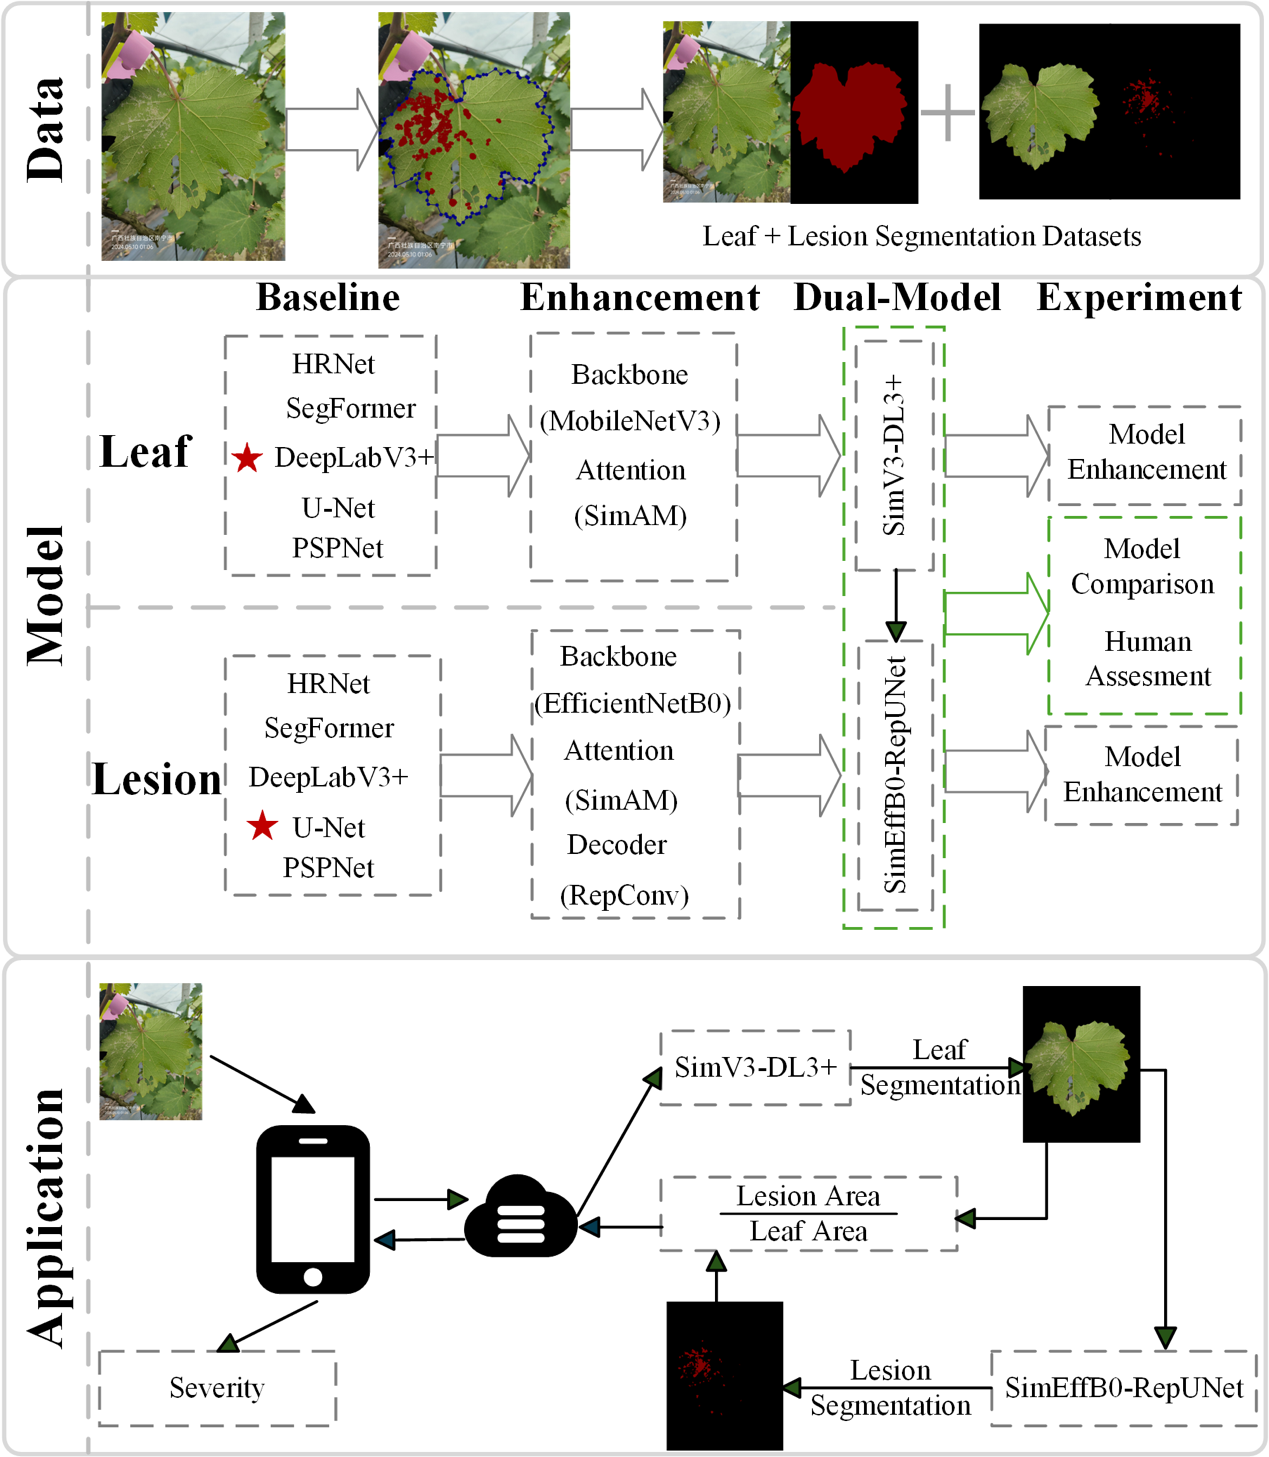
\includegraphics[width=5.76806in,height=6.62083in]{DSLL-Net-media/media/image1.png}

Fig. 1. The overall research workflow involving data, model and
application. The upper section illustrates the complete pipeline for
data preprocessing and dataset construction. The middle section
highlights the architectural design and enhancements of the leaf and
lesion segmentation model in the dual-stage model, with a star (\(\star\))
marking the selected baseline models after rigorous comparative
evaluation. The lower section presents the workflow of a mobile
application based on our dual-stage model, which clearly demonstrates
how the severity can be obtained by the model enabled mobile application
system in practical use.

\hypertarget{data-preparation}{%
\subsection{Data Preparation}\label{data-preparation}}

A total of 696 field images were collected between April and August 2024
at two sites (Mingyang and Du'an) in Guangxi, China. Images were
captured using a Huawei P70 and an iPhone 15 at a camera-to-subject
distance of 15--20 cm, with each image focused on a single leaf. To
ensure data quality and consistency, images were selected under
controlled illumination conditions (excluding strong direct sunlight),
with naturally oriented leaves, appropriate viewing angles, and clearly
visible, intact leaf structures free from occlusion.

Manual annotations were conducted using LabelMe (v3.16.7) to precisely
delineate leaf regions and disease lesions
(https://github.com/wkentaro/labelme.git). From these annotations, two
binary masks were generated for each image: a leaf mask (leaf vs.
background) and a lesion mask (lesion vs. non-lesion). These labeled
data were further used to construct three task-specific datasets for
different modeling strategies, as summarized in Table. 1

Table. 1 An overview of the constructed datasets and their corresponding
modeling tasks.

\begin{longtable}[]{@{}llllll@{}}
\toprule
Dataset & Input to model & Label(s) & Construction & Task & Models using
it \\
\midrule
\endhead
Leaf segmentation & Original full RGB field image & Leaf mask (binary) &
Manual annotation on original image & Leaf extraction from background &
Stage-1 models: DeepLabV3+ (baseline comparisons), SimV3-DL3+ \\
Lesion segmentation & Cropped leaf ROI & Lesion mask (binary, cropped
consistently) & Crop leaf regions using leaf masks; pair with cropped
lesion masks & Fine-grained lesion segmentation within leaf & Stage-2
models: U-Net family, SimEffB0-RepUNet \\
Single-stage segmentation & Original full RGB field image & Lesion mask
(binary) & Original images + lesion masks & Single-stage lesion
segmentation & Single-stage baselines: U-Net, DeepLabV3+, PSPNet, HRNet,
SegFormer \\
\bottomrule
\end{longtable}

To guarantee experimental consistency, a fixed train--test partition
(567 training and 129 testing images; 80\%/20\%) was enforced across all
dataset variants. To simulate practical deployment conditions, the
lesion model in the second stage was conditioned on predicted leaf masks
produced by the first-stage segmentation model, rather than relying on
ground-truth annotations.

\hypertarget{dual-stage-segmentation-model}{%
\subsection{Dual-Stage Segmentation
Model}\label{dual-stage-segmentation-model}}

\hypertarget{leaf-segmentation-model-simv3-dl3}{%
\subsection{Leaf Segmentation Model
SimV3-DL3+}\label{leaf-segmentation-model-simv3-dl3}}

Leaf regions, characterized by larger spatial extent and clearer
structural boundaries, are inherently easier to segment than lesions,
typically leading to higher segmentation accuracy. Accordingly, the
first-stage model prioritizes a balance between accuracy and a
lightweight design to enable efficient deployment on mobile devices in
field environments. To establish a suitable baseline, five
representative semantic segmentation models---DeepLabV3+ {[}17{]},
U-Net{[}18{]}, PSPNet {[}19{]}, SegFormer {[}20{]}, and HRNet
{[}21{]}---were comparatively evaluated. As shown in Fig. 4, DeepLabV3+
achieved the best overall performance, offering the highest accuracy
with a moderate model size, and was therefore selected as the baseline.

In its lightweight configuration, DeepLabV3+ is typically coupled with a
MobileNet backbone to achieve a favorable balance between accuracy and
efficiency. Owing to their efficiency--accuracy trade-off, MobileNet
architectures are widely adopted in mobile vision applications
{[}28-29{]}. MobileNetV2 employs inverted residual blocks with linear
bottlenecks to reduce computational cost {[}23{]}, yet its
representational capacity is often insufficient for capturing
fine-grained boundaries in heterogeneous field conditions. MobileNetV3
addresses this limitation by integrating squeeze-and-excitation (SE)
modules and hard-swish activations, enhancing feature representation
while preserving efficiency. More recent variants such as MobileNetV4,
designed via neural architecture search with compound scaling, offer
further accuracy gains but introduce increased structural complexity and
training overhead {[}24{]}. In view of practical deployment constraints,
MobileNetV3 was selected as the backbone of the proposed model.

While the SE attention mechanism in MobileNetV3 improves feature
representation with relatively low computational cost, it introduces
additional parameters and inadequately captures spatial structures
essential for pixel-level segmentation, as its design focuses on
inter-channel dependencies via global pooling and lightweight fully
connected layers {[}25{]}. In contrast, the Simple, Parameter-Free
Attention Module (SimAM) adopts a parameter-free formulation that
directly modulates neuron responses based on spatial significance,
enabling more effective modeling of fine-grained structural patterns
{[}26{]}. This characteristic is particularly beneficial for
leaf--lesion scenarios, where subtle spatial variations and boundary
details play a critical role. By integrating SimAM, the network is able
to better capture discriminative regions within grape leaves while
suppressing irrelevant background interference. Importantly, the absence
of additional learnable parameters allows SimAM to preserve the
computational efficiency of the MobileNetV3 backbone, making it
well-suited for real-time and resource-constrained deployment. Based on
these considerations, SimAM is employed to replace the SE module in the
final leaf segmentation model.

Guided by the above design considerations, a leaf segmentation model is
constructed, with its overall architecture presented in Fig. 2\textbf{.}

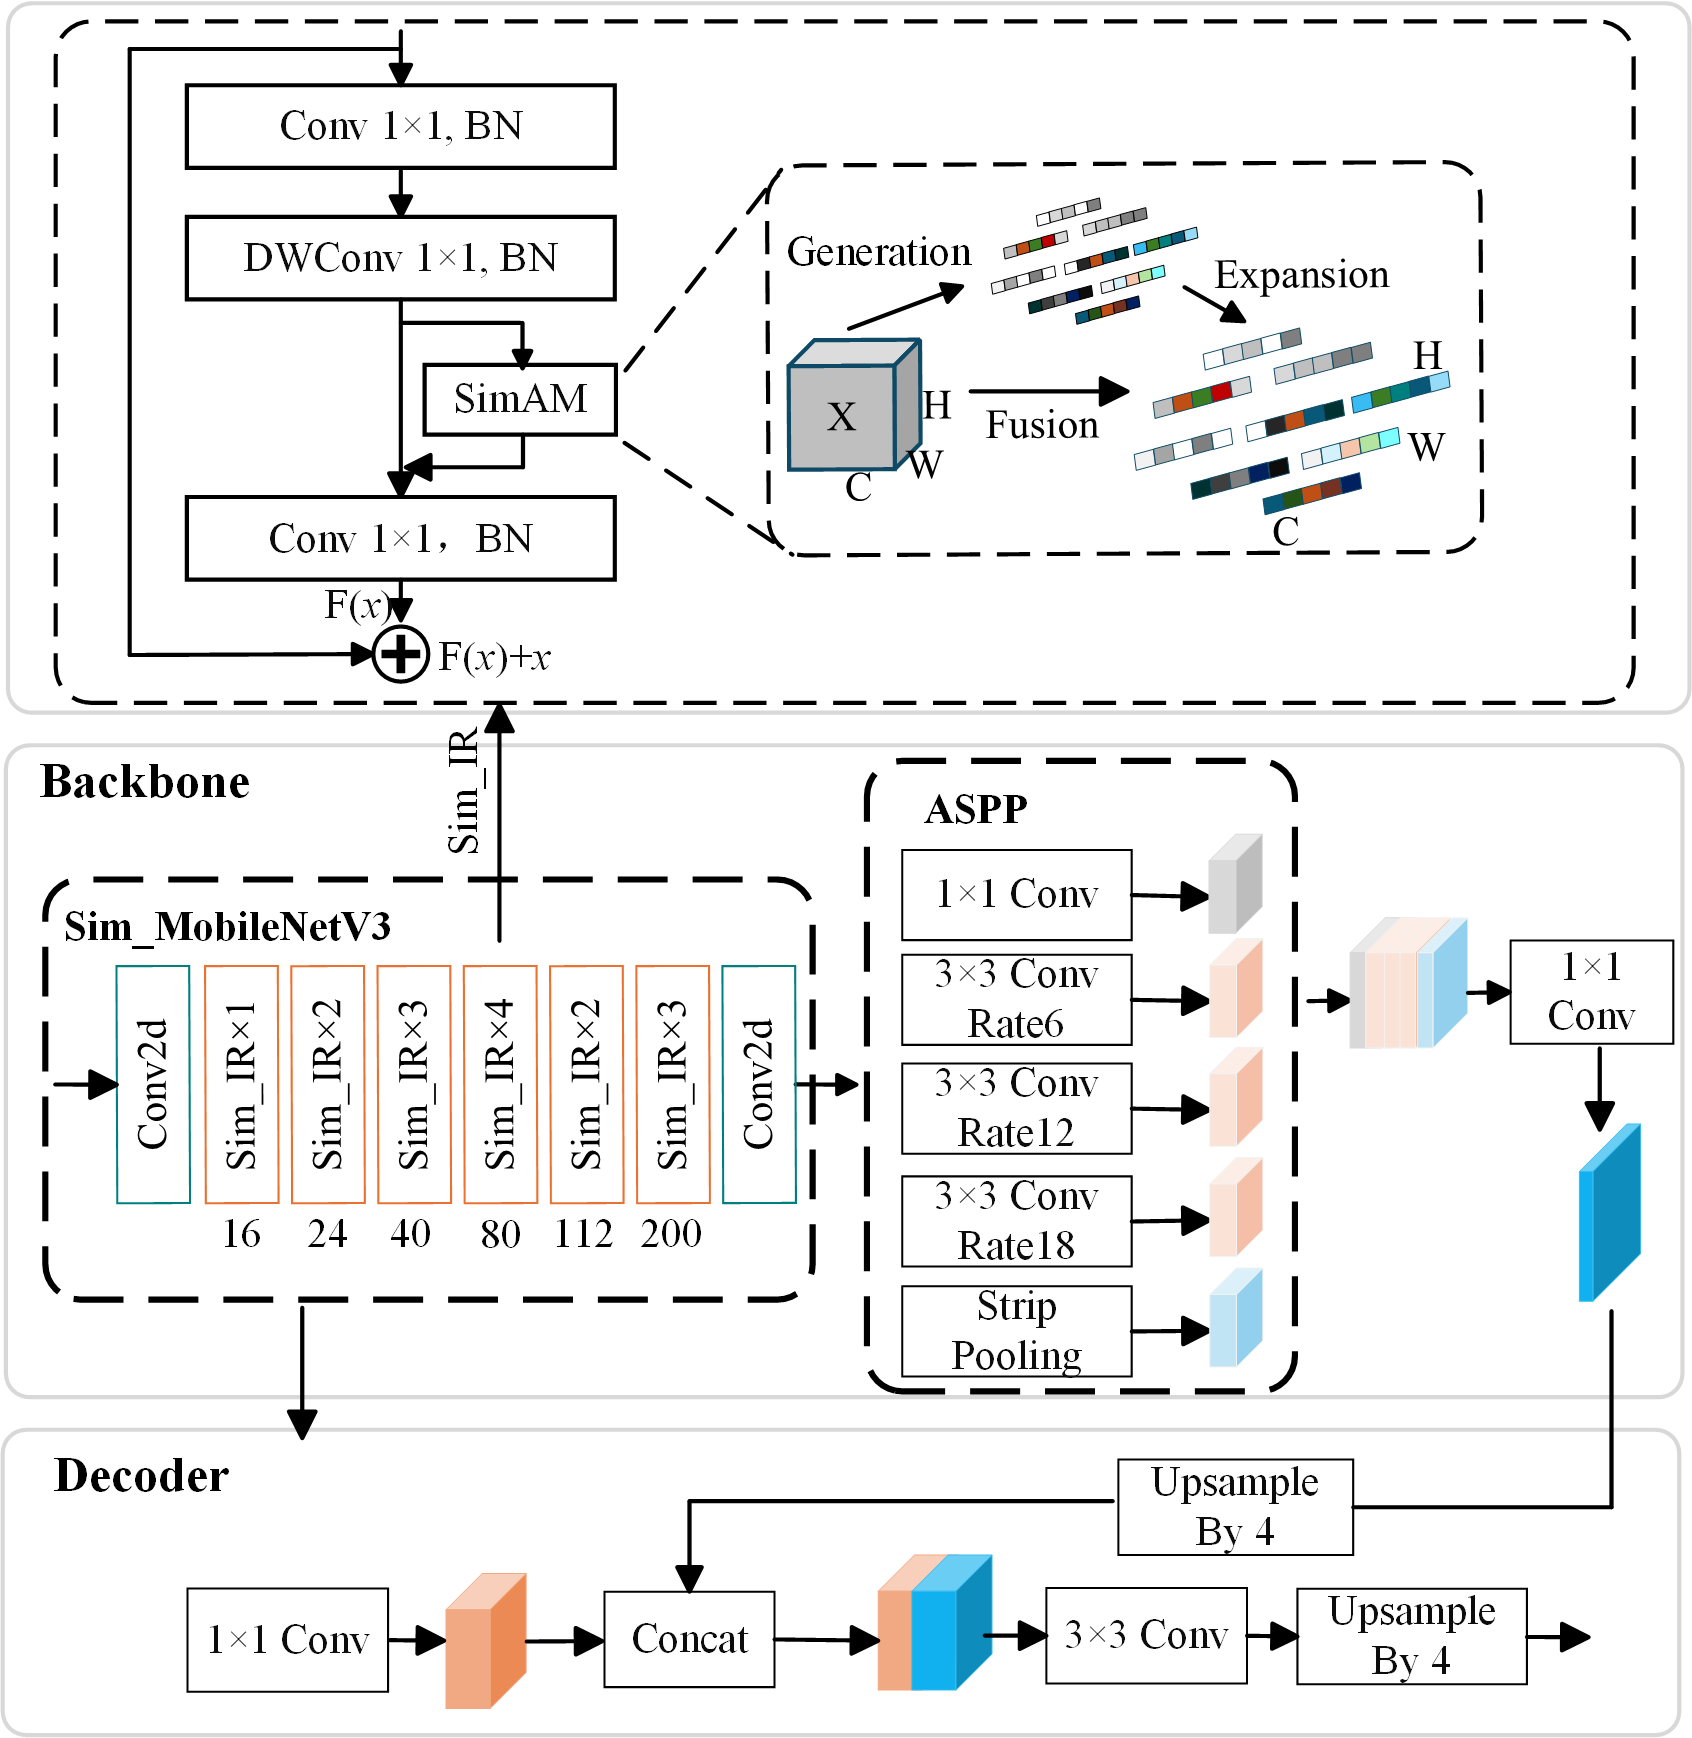
\includegraphics[width=5.63889in,height=5.79167in]{DSLL-Net-media/media/image2.png}

Fig. 2. Architecture of the SimV3-DL3+ Model. The backbone and decoder
present the overall architecture of SimV3-DL3+. Sim\_IR denotes the
module obtained by enhancing the original InvertedResidual block with
the SimAM attention. The upper part shows the detailed structure of the
SimIR module and the computational flow of the SimAM attention.

\hypertarget{lesion-segmentation-model-simeffb0-repunet}{%
\subsection{\texorpdfstring{Lesion Segmentation Model (SimEffB0-RepUNet)
}{Lesion Segmentation Model (SimEffB0-RepUNet) }}\label{lesion-segmentation-model-simeffb0-repunet}}

Given the inherent difficulty of lesion segmentation, achieving high
accuracy is prioritized in the model design. Accordingly, the model is
first optimized for segmentation performance, after which efficiency and
parameter reduction are further considered.

To construct a reliable lesion segmentation model for the second stage,
five representative architectures---DeepLabV3+, U-Net, PSPNet,
SegFormer, and HRNet---were systematically evaluated on the lesion
dataset. Among these candidates, U-Net exhibited the highest
segmentation accuracy, despite its relatively high parameter cost, and
was selected as the baseline for subsequent model development. In
standard practice, U-Net is commonly implemented with a VGG16 encoder.

Although this configuration ensures stable performance, the associated
parameter overhead limits its efficiency in deployment scenarios with
constrained computational resources. To address this limitation, the
encoder was reconfigured using EfficientNet-B0, which adopts a compound
scaling strategy across network dimensions to achieve more efficient
feature representation with reduced complexity. This design is
particularly effective for capturing the subtle texture and structural
variations characteristic of small and irregular lesion regions.

The encoder adopts EfficientNet-B0, whose architecture is composed of
stacked MBConv blocks with integrated squeeze-and-excitation (SE)
attention in its original design. Following the design in the leaf
segmentation stage, the SE module is replaced with the Simple Attention
Module (SimAM) to improve spatial feature representation without
increasing model complexity{[}26{]}. This adjustment enhances the
modeling of fine-grained lesion patterns and reduces background
interference, while maintaining the lightweight and efficient
characteristics of the encoder.

In the decoder, although multi-scale features are progressively
reconstructed through upsampling and skip connections, the fusion
process can still result in boundary ambiguity and limited structural
coherence, especially for small and irregular lesions. To mitigate this
issue, RepConv blocks based on structural re-parameterization {[}27{]}
are incorporated into the upsampling pathway to strengthen feature
integration. RepConv leverages a multi-branch convolutional structure
during training to enhance representational capacity, which is
subsequently re-parameterized into a single convolutional operation for
inference. This design facilitates more accurate reconstruction of
lesion boundaries without introducing additional computational overhead
at deployment. Based on these considerations, RepConv is incorporated
into the decoder.

In summary, the proposed lesion segmentation model, termed
SimEffB0-RepUNet, integrates a SimAM-enhanced EfficientNet-B0 encoder
with a RepConv-based decoder within the U-Net framework. This design is
intended to improve the segmentation of small and irregular lesions
while maintaining computational efficiency suitable for practical field
deployment. The overall architecture of SimEffB0-RepUNet is shown in
Fig. 3\textbf{.}

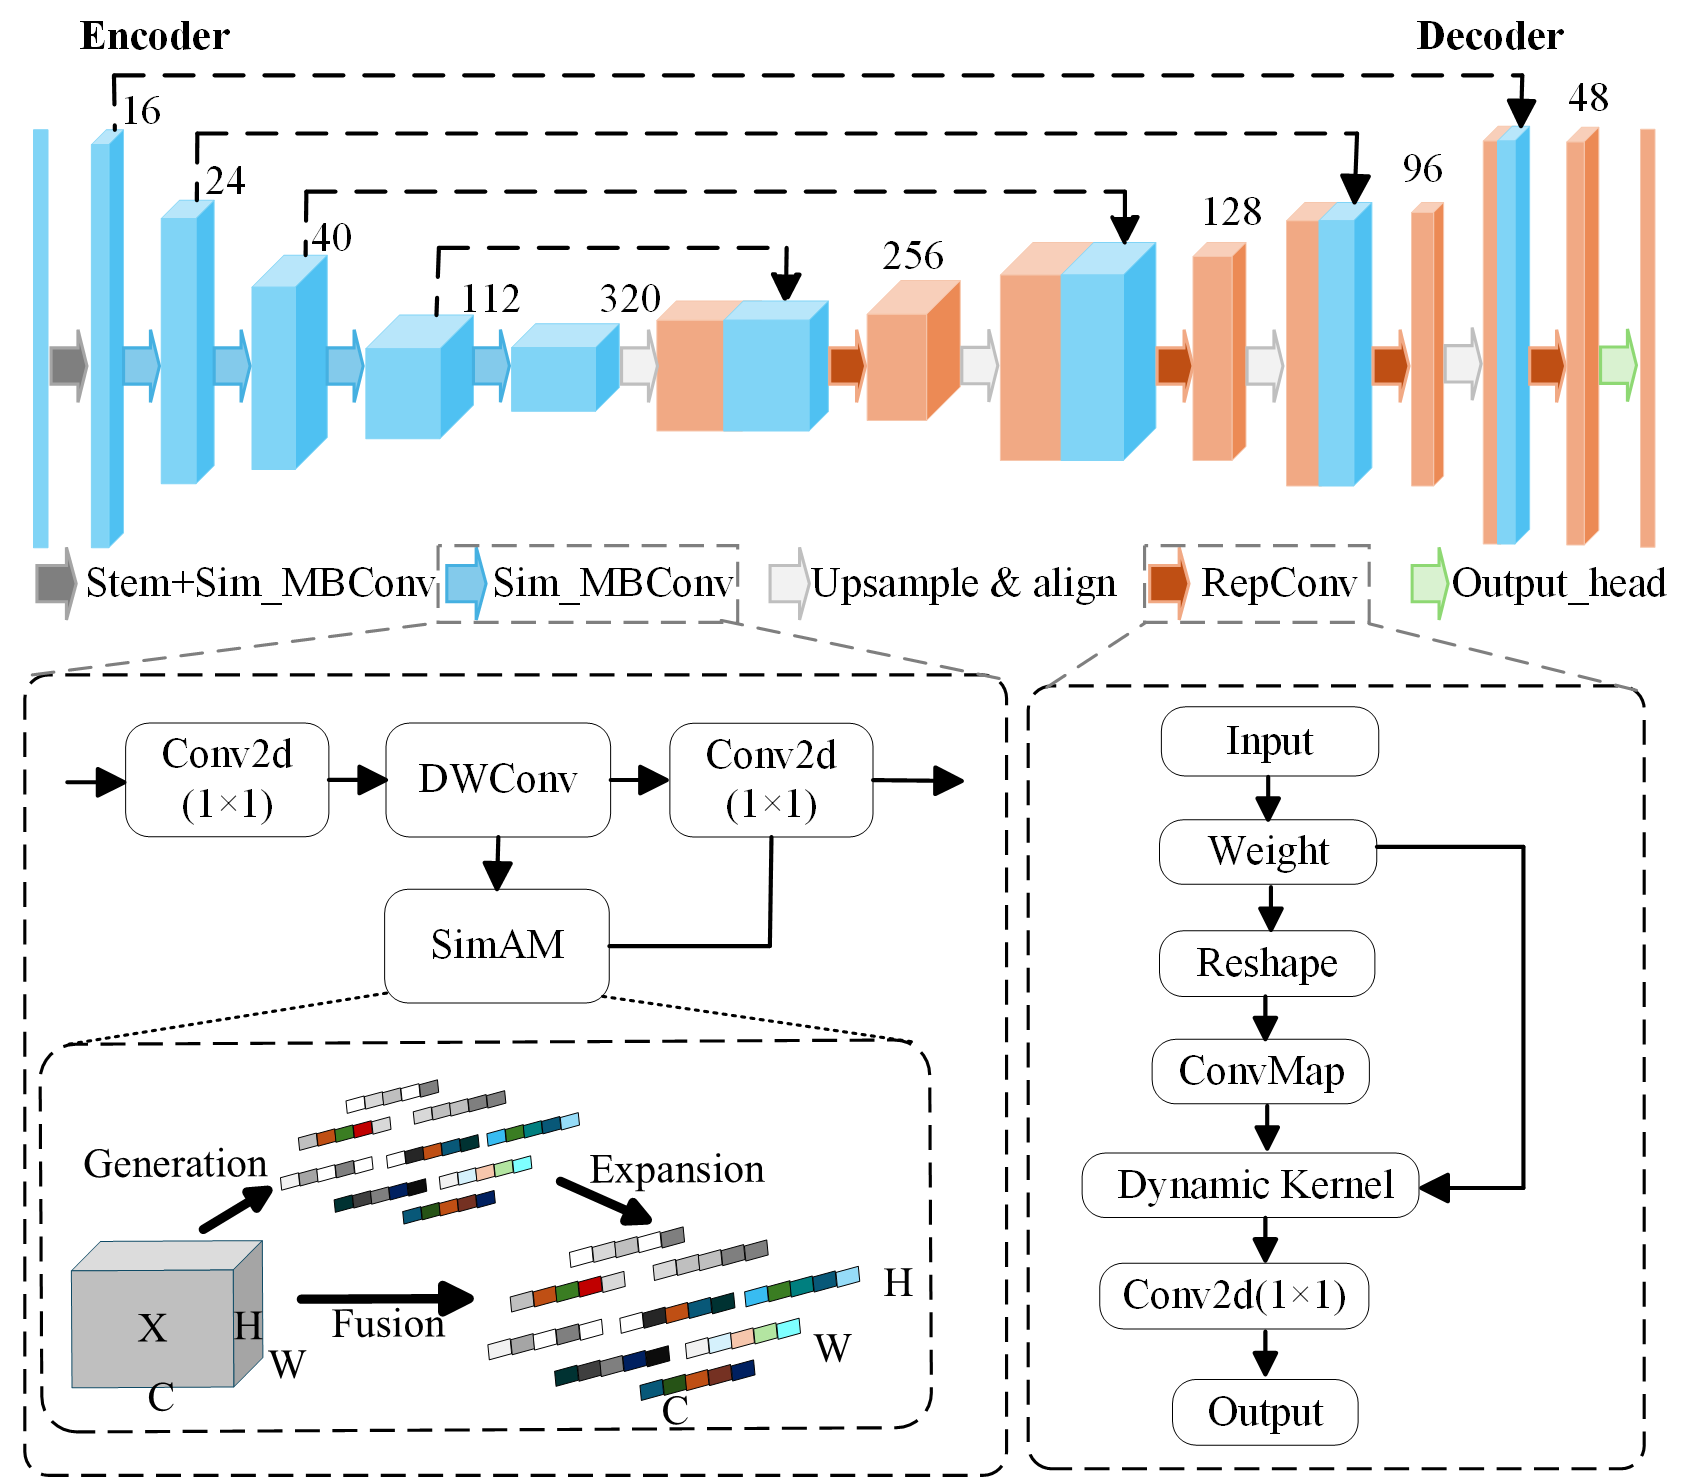
\includegraphics[width=5.625in,height=4.91667in]{DSLL-Net-media/media/image3.png}

Fig. 3. Architecture of the proposed SimEffB0-RepUNet model. The upper
part shows the overall structure of SimEffB0-RepUNet, which is built
upon the U-Net framework, using EfficientNetB0 with embedded SimAM
attention as the encoder and RepConv modules in the decoder. The lower
left illustrates the structure of the Sim\_MBConv enhanced by the SimAM
mechanism, while the lower right presents the architecture of the
RepConv module. Sim\_MBConv refers to an EfficientNetB0 block enhanced
by SimAM.

\hypertarget{experimental-design}{%
\subsection{Experimental design}\label{experimental-design}}

\hypertarget{leaf-segmentation}{%
\subsection{Leaf segmentation}\label{leaf-segmentation}}

To identify a suitable baseline model that best balances leaf
segmentation accuracy and computational efficiency, five representative
semantic segmentation architectures---U-Net, DeepLabV3+, PSPNet, HRNet,
and SegFormer---were comparatively evaluated on the leaf segmentation
task. Performance was assessed using six key metrics, including Mean
Pixel Accuracy (mPA), Intersection over Union for the background and
leaf regions (IoU-Background, IoU-Leaf), Mean Intersection over Union
(mIoU), the number of model parameters (Params), and the inference time.
Here, IoU-Background corresponds to the overlap over non-leaf regions,
i.e., areas outside the leaf mask. Among these metrics, IoU-Leaf is
treated as the primary evaluation criterion, as it directly reflects the
accuracy of leaf region delineation.

To examine the effect of backbone selection, five lightweight
networks---MobileNetV2 (baseline), MobileNetV3, MobileNetV4 {[}24{]},
StarNetS1 {[}28{]}, and EfficientNetB0---were incorporated into the
baseline architecture for comparative evaluation. All MobileNet variants
were implemented in their large configurations. The evaluation followed
the same metric setting as the baseline analysis, ensuring a consistent
comparison of efficiency--accuracy trade-offs across different
backbones.

To examine the contribution of SimAM to spatial feature representation,
a comparative study was performed within the DeepLabV3+ framework by
replacing the original squeeze-and-excitation (SE) attention with SimAM
in the MobileNetV3 backbone. The resulting variants---SimAM-enhanced
MobileNetV3 (Sim-MobileNetV3) and the original MobileNetV3 with SE
{[}25{]}---were evaluated under an identical metric setting to ensure a
fair assessment of their impact on leaf segmentation performance.

\hypertarget{lesion-segmentation}{%
\subsection{Lesion segmentation}\label{lesion-segmentation}}

A series of experiments were designed to systematically evaluate lesion
segmentation performance. As an initial step, four representative
models---U-Net, DeepLabV3+, PSPNet, and HRNet---were comparatively
evaluated under the same protocol as used in the leaf segmentation task
to establish a suitable baseline architecture. Performance was measured
using five metrics, including mean pixel accuracy (mPA), intersection
over union for background and lesion regions (IoU-Background and
IoU-Disease), mean intersection over union (mIoU), model parameters, and
inference time. Among these, IoU-Disease is treated as the primary
evaluation criterion due to its direct relevance to lesion delineation
accuracy, while IoU-Background corresponds to the overlap over
non-lesion regions.

Subsequently, to examine the effect of backbone enhancement, six
commonly used architectures------VGG16, ResNet50 {[}21{]} , ResNetRS50
{[}29{]}, MobileNetV2, MobileNetV3, and EfficientNetB0---were
incorporated into the baseline model for comparative evaluation.

Following this, the role of attention mechanisms was further
investigated by comparing SimAM with three widely used modules--- SE,
ECA {[}30{]}, and CBAM {[}31{]}. The comparison focuses on their
capability to enhance both spatial and channel-wise feature
representations and their impact on lesion segmentation performance.

Finally, the contribution of the RepConv-based decoder was assessed by
replacing the original double-convolution module with several
representative alternatives, including standard convolution, RepConv,
ODConv {[}32{]}, PConv {[}33{]}, and CondConv2D {[}34{]} modules. The
comparison focuses on their ability to preserve spatial details during
feature reconstruction, evaluated using mPA, IoU-disease, parameter
count, and inference time.

\hypertarget{model-comparison-experiments}{%
\subsection{Model Comparison
Experiments}\label{model-comparison-experiments}}

To further investigate the effectiveness of the proposed dual-stage
strategy for lesion extraction, three segmentation
paradigms---single-stage, conventional dual-stage, and the proposed
dual-stage approach---were comparatively analyzed. For the single-stage
setting, five representative architectures---U-Net, DeepLabV3+, PSPNet,
HRNet, and SegFormer---were trained and evaluated on the corresponding
dataset, where lesion segmentation is performed directly without an
explicit prior leaf segmentation step.

For the dual-stage setting, a conventional configuration was constructed
using DeepLabV3+ (MobileNetV2) for leaf segmentation followed by U-Net
(VGG16) for lesion segmentation, serving as a representative baseline.
This configuration was further compared with the proposed dual-stage
framework, SimV3-DL3+ + SimEffB0-RepUNet, in which leaf and lesion
segmentation are explicitly decoupled and optimized through dedicated
models at each stage.

Model performance was assessed using four metrics: inference time,
parameter count, intersection over union for leaf regions (IoU-Leaf),
and intersection over union for lesion regions (IoU-Disease). Inference
time here is defined as the average processing time per image, computed
by dividing the total inference time over the test set by the number of
test samples. For dual-stage models, this measure additionally accounts
for the sequential execution of both stages, including leaf and lesion
prediction, intermediate processing (e.g., pixel counting), and data
transfer between stages. This evaluation enables a comprehensive
comparison of segmentation accuracy and computational efficiency across
different modeling strategies.

\hypertarget{expert-visual-evaluation-and-model-prediction}{%
\subsection{Expert Visual Evaluation and Model
Prediction}\label{expert-visual-evaluation-and-model-prediction}}

To compare model-based severity estimation with human expert judgment, a
visual evaluation experiment was conducted involving trained
technicians. A total of 15 technicians with formal training and
practical experience in crop disease diagnosis were included, all of
whom were familiar with symptom recognition and field-based severity
assessment.

Each technician independently evaluated the leaf images and estimated
disease severity based on visual inspection, without the aid of
quantitative tools. In parallel, the proposed model generated automated
severity predictions for the same image set. The resulting expert
assessments and model outputs were subsequently compared to examine
their consistency and to assess the potential of the model to provide
more objective, reproducible, and scalable severity estimation.

\hypertarget{experimental-setup}{%
\subsection{Experimental setup}\label{experimental-setup}}

All experiments were performed on a workstation equipped with an NVIDIA
GeForce RTX 4060 Ti GPU (16 GB memory) and an Intel® Core™ i5-13490F CPU
(2.50 GHz), with 32 GB RAM, running Python 3.8 on a 64-bit Windows 10
operating system with CUDA 11.8. The models were trained using the Adam
optimizer with a batch size of 2. The initial learning rate was set to
\(1 \times 10^{-5}\) and adjusted using a cosine annealing schedule, with a minimum
value of \(1 \times 10^{-6}\) to ensure stable convergence in later training stages.
All input images were resized to \(512 \times 512\) pixels prior to training, and
the models were trained for 500 epochs. Dice loss function was adopted
as the objective function, formulated as \(\left( 1 \right)\)

\begin{equation}
\mathcal{L}_{D\text{ice}} = 1 - \frac{2|X \cap Y|}{\left| X \right| + |Y|}
\tag{1}
\end{equation}

where \(X\) and \(Y\)denote the predicted and ground truth masks. It
measures the overlap between the two sets, encouraging higher similarity
and effectively addressing class imbalance in segmentation tasks.

\hypertarget{evaluation-metrics}{%
\subsection{Evaluation metrics}\label{evaluation-metrics}}

To quantitative evaluate the segmentation performance, several standard
metrics are employ. Pixel Accuracy (PA) provides a global perspective by
calculating the fraction of correctly identified pixels::

\begin{equation}
PA = \frac{\sum_{i = 0}^{k}P_{\text{ii}}}{\sum_{i = 0}^{k}{\sum_{j = 0}^{k}P_{\text{ij}}}}
\tag{2}
\end{equation}

where \(P_{\text{ii}}\) is the number of pixels correctly classified as
class \(i\), and \(P_{\text{ij}}\) is the number of pixels whose
ground-truth class is \(i\) but predicted as class \(j\) (\(i \neq j\)).

Beyond global accuracy, Mean Pixel Accuracy (mPA) offers a more
class-aware evaluation by averaging the individual accuracies across all
categories:

\begin{equation}
\text{mPA} = \frac{1}{K + 1}\sum_{i = 0}^{K}\frac{P_{\text{ii}}}{\sum_{j = 0}^{K} P_{\text{ij}}}
\tag{3}
\end{equation}

Here, K denotes the number of foreground classes in the segmentation
task, and \emph{K+1} represents the total number of classes including
the background.

The Intersection over Union (IoU), or the Jaccard Index, further
characterizes the spatial overlap between the prediction and ground
truth, which is formulated:

\begin{equation}
\text{IoU}_{i} = \frac{TP_{i}}{TP_{i} + FP_{i} + FN_{i}}
\tag{4}
\end{equation}

where \(TP_{i}\), \(FP_{i}\), and \(FN_{i}\) denote the numbers of
true-positive, false-positive, and false-negative pixels for class
\(i\), respectively.

To provide a consolidated performance metric across the entire dataset,
the Mean Intersection over Union (mIoU) is synthesized by aggregating
the IoU values across all semantic categories:

\begin{equation}
\text{mIoU} = \frac{1}{K + 1}\sum_{i = 0}^{K}\text{IoU}_{i}
= \frac{1}{K + 1}\sum_{i = 0}^{K}\frac{TP_{i}}{TP_{i} + FP_{i} + FN_{i}}
\tag{5}
\end{equation}

To quantify the regression performance and the degree of linear
correlation between the observations and predictions, the coefficient of
determination (\(R^{2}\)) is employed. It encapsulates the proportion of
total response variance that is captured by the proposed model. A
\(R^{2}\) value approaching unity signifies a superior goodness-of-fit,
reflecting that the model effectively accounts for the underlying data
variability The mathematical representation is given as Equation
(\(6\)).

\begin{equation}
R^{2} = 1 - \frac{\sum_{i = 1}^{n}\left( y_{i} - {\widetilde{y}}_{i} \right)^{2}}{\sum_{i = 1}^{n}\left( y_{i} - \bar{y} \right)^{2}}
\tag{6}
\end{equation}

where \(n\) is the number of samples, \(y_{i}\) and
\({\widetilde{y}}_{i}\ \)are the actual and predicted values,
respectively, and \(\bar{y}\) is the mean of all actual values.

To evaluate the average prediction discrepancy in the same units as the
target variable, the Mean Absolute Error (MAE) is utilized. Unlike
metrics that square the deviations, MAE provides a linear representation
of the error magnitude, offering a resilient measure against outliers
that does not account for the direction of the residuals, as shown in
Equation (\(7\)).

\begin{equation}
\text{MAE} = \frac{1}{n}\sum_{i = 1}^{n}{|y_{i} - {\widetilde{y}}_{i}|}
\tag{7}
\end{equation}

The Root Mean Squared Error (RMSE) serves as a quadratic loss metric
that quantifies the standard deviation of the prediction residuals. By
taking the square root of the average squared discrepancies, RMSE
inherently assigns a disproportionate weight to larger errors, thereby
offering heightened sensitivity to outliers compared to MAE. RMSE is
especially useful when large deviations are particularly undesirable, as
shown in Equation \(1\).

\begin{equation}
\text{RMSE} = \sqrt{\frac{1}{n}\sum_{i = 1}^{n}{(y_{i} - {\widetilde{y}}_{i})}^{2}}
\tag{8}
\end{equation}

\hypertarget{results}{%
\section{Results}\label{results}}

\hypertarget{leaf-segmentation-1}{%
\subsection{Leaf segmentation}\label{leaf-segmentation-1}}

The comparative results of baseline model evaluation for leaf
segmentation are shown in Fig. 4. Among the five evaluated models,
DeepLabV3+ achieved the best overall segmentation performance,
outperforming the other architectures across all accuracy-related
metrics. Specifically, DeepLabV3+ reached an mPA of 99.11\%, IoU values
of 98.70\% for background and 97.49\% for leaf regions, and an mIoU of
98.09\%. In addition to its high accuracy, DeepLabV3+ exhibited a
moderate model size and an inference time that was second only to
PSPNet, indicating a favorable balance between accuracy and efficiency.

HRNet achieved the second-highest segmentation accuracy across most
metrics; however, this improvement came at the cost of a substantially
larger model size and longer inference time, which limits its
suitability for efficient field deployment. U-Net ranked third in
segmentation accuracy but exhibited the largest parameter count and the
longest inference time among the five models. PSPNet achieved relatively
lower accuracy---only outperforming SegFormer---while offering the
smallest model size and the fastest inference speed. SegFormer showed
the lowest segmentation accuracy overall, despite maintaining a compact
architecture and moderate inference time.

Considering both segmentation accuracy and computational efficiency,
DeepLabV3+ demonstrated the most favorable overall performance among the
evaluated models and was therefore selected as the baseline architecture
for subsequent experiments.

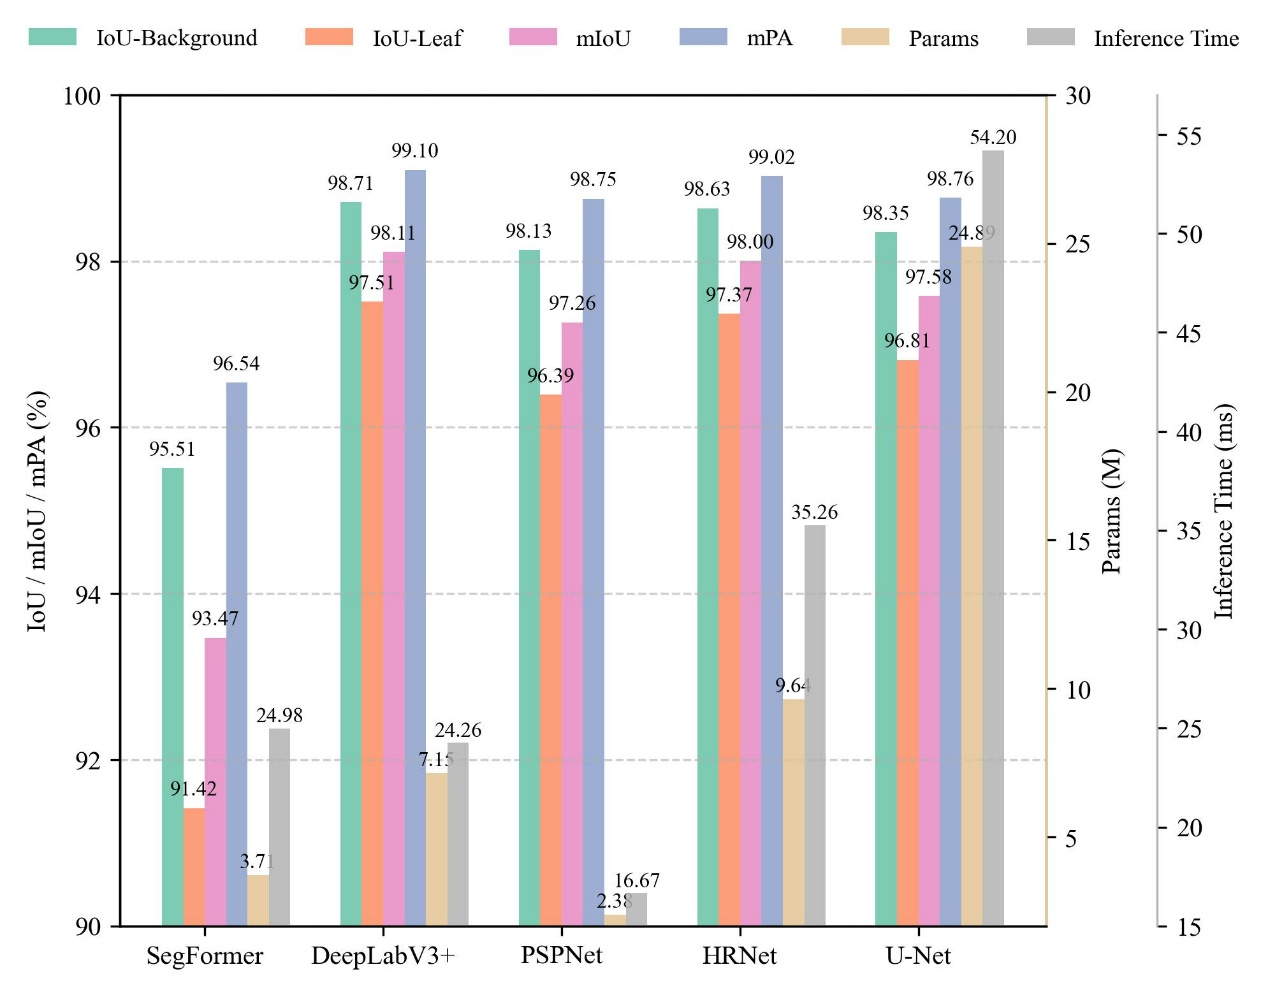
\includegraphics[width=5.76806in,height=4.49514in]{DSLL-Net-media/media/image4.jpeg}

Fig. 4. Performance comparison of five semantic segmentation models for
leaf segmentation---SegFormer, DeepLabV3+, PSPNet, HRNet, and
U-Net---evaluated using segmentation accuracy metrics, parameter count,
and inference time.

Fig. 5 shows the performance of DeepLabV3+ with different backbones for
leaf segmentation. Using MobileNetV2, the baseline model achieved an mPA
of 99.10\% and an mIoU of 98.11\%, with 7.15 M parameters and 20.43
ms(millisecond) inference time. MobileNetV3 slightly improved accuracy
with fewer parameters but longer inference time (25.65 ms), while
MobileNetV4 resulted in reduced accuracy with increased model size and
latency. StarNet-S1 exhibited the lowest accuracy but maintained
relatively fast inference. EfficientNet-B0 achieved accuracy comparable
to the baseline but incurred the largest parameter count and the
second-longest inference time. In contrast, Sim\_MobileNetV3 achieved
the best overall performance, reaching the highest mPA (99.19\%) and
mIoU (98.30\%) with the smallest model size (4.83 M) and a fast
inference time (20.62 ms).
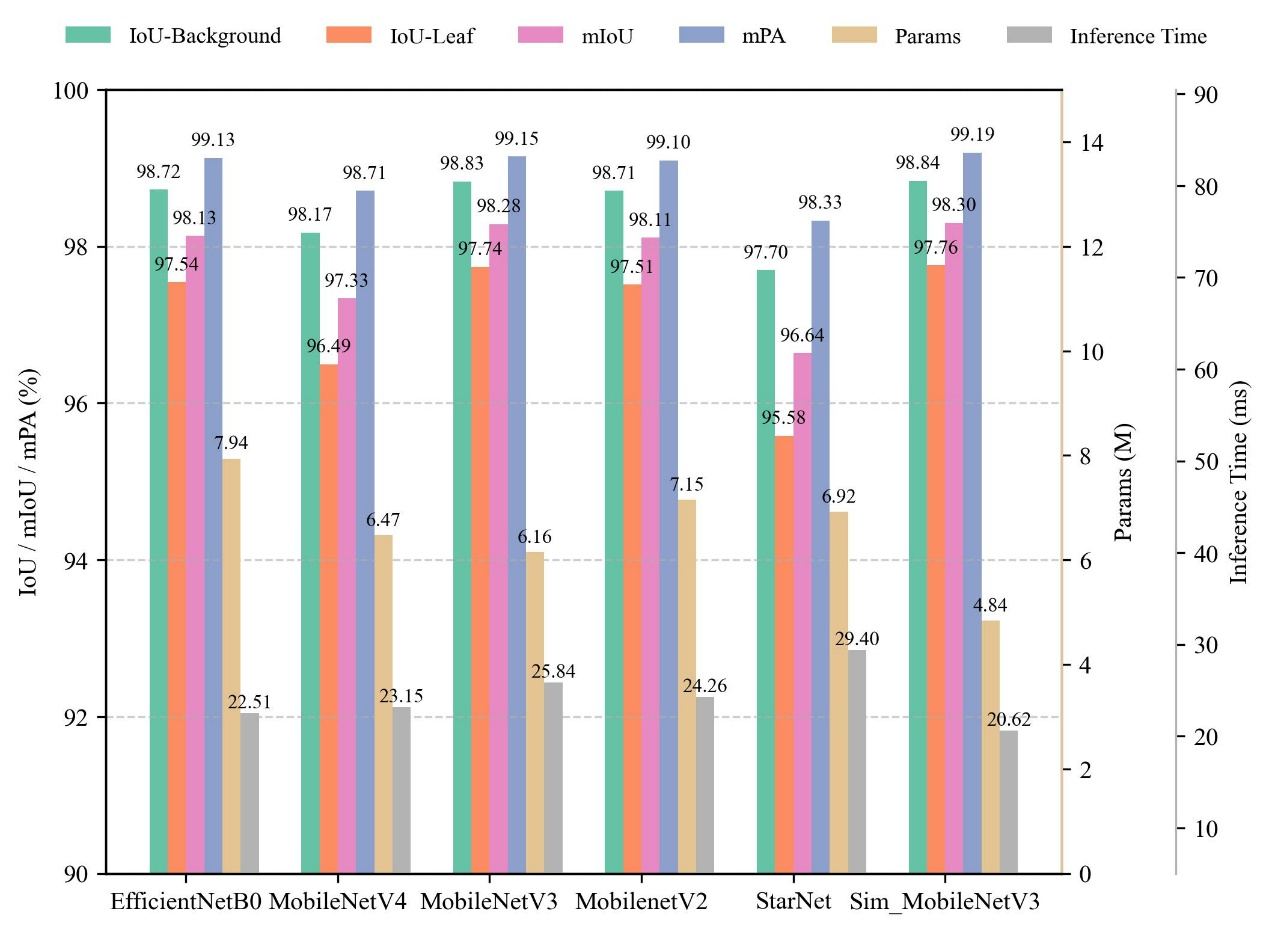
\includegraphics[width=5.76806in,height=4.23194in]{DSLL-Net-media/media/image5.jpeg}

Fig. 5. Leaf segmentation performance of DeepLabV3+ models with
different backbone networks, including EfficientNet-B0, MobileNetV4,
MobileNetV3, MobileNetV2 (baseline), StarNet, and Sim\_MobileNetV3.
Models are evaluated using segmentation accuracy metrics, parameter
count, and inference time.

\hypertarget{lesion-segmentation-1}{%
\subsection{Lesion segmentation}\label{lesion-segmentation-1}}

Fig. 6 compares the lesion segmentation performance of five semantic
segmentation models: U-Net, HRNet, PSPNet, DeepLabV3+, and SegFormer.
U-Net achieved the highest segmentation accuracy, with an mIoU of
84.97\%, IoU-Disease of 73.07\%, IoU-Background of 96.87\%, and mPA of
91.38\%, but also exhibited the largest parameter count (24.89 M) and
the longest inference time (51.53 ms). HRNet achieved slightly lower
accuracy (mIoU 84.86\%, IoU-Disease 72.86\%) with fewer parameters (9.64
M) and moderate inference time (35.26 ms). DeepLabV3+ showed competitive
accuracy (mIoU 84.09\%, IoU-Disease 71.42\%) with a smaller model size
(7.15 M) and faster inference (22.26 ms). SegFormer achieved moderate
performance (mIoU 80.79\%, IoU-Disease 65.46\%) with 13.68 M parameters,
while PSPNet exhibited the lowest accuracy (mIoU 71.72\%, IoU-Disease
51.35\%) but the smallest model size (2.38 M) and fastest inference
(17.10 ms). Overall, U-Net provided the best lesion segmentation
accuracy and was therefore selected as the baseline model for subsequent
experiments.

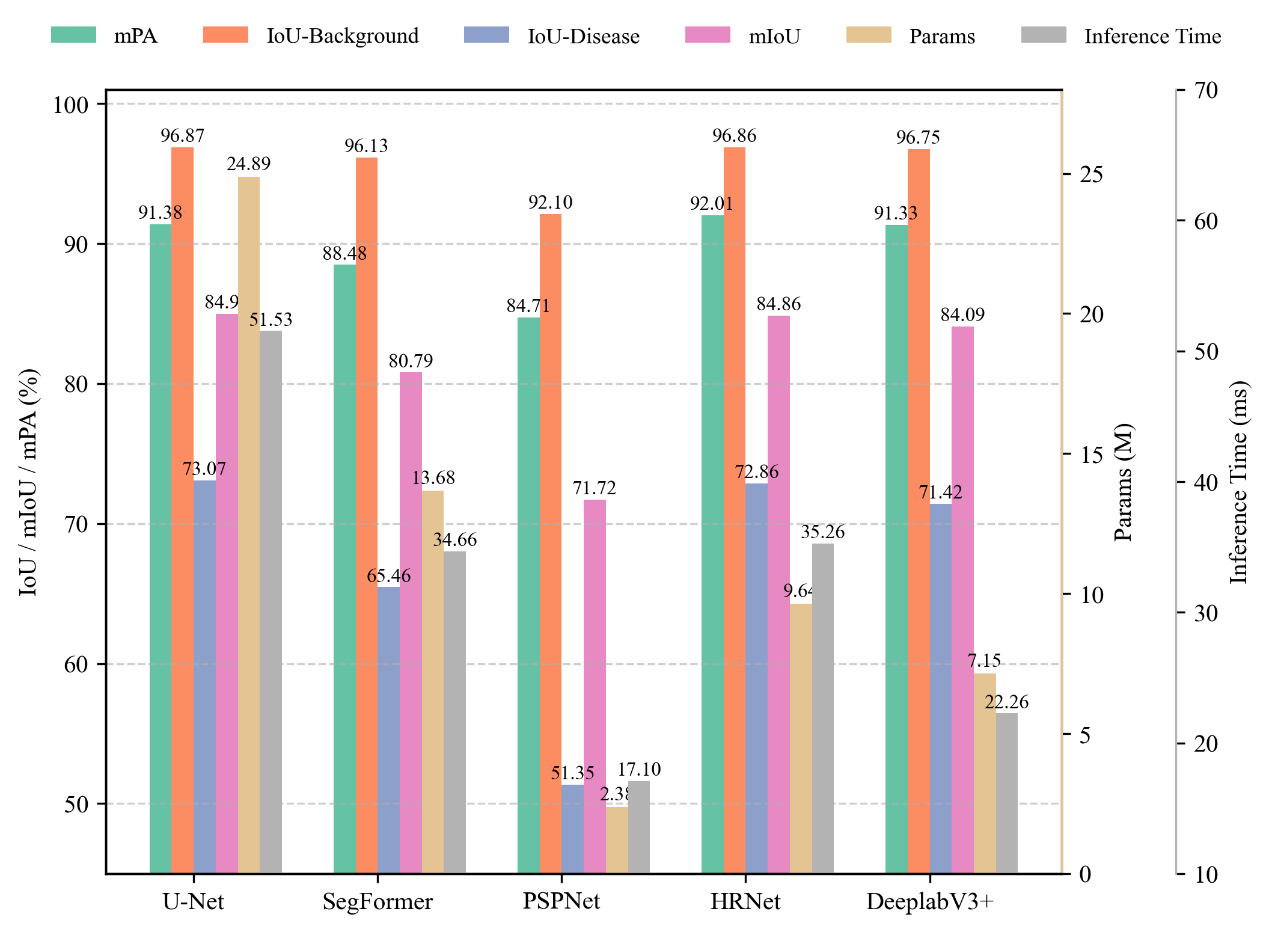
\includegraphics[width=5.76806in,height=4.23611in]{DSLL-Net-media/media/image6.png}

Fig. 6. Lesion segmentation performance of five semantic segmentation
models---U-Net, SegFormer, PSPNet, HRNet, and DeepLabV3+,---evaluated
using mPA, IoU-Background, IoU-Disease, mIoU, parameter count, and
inference time.

Fig. 7 presents the lesion segmentation performance of the U-Net model
with different backbone networks, including VGG16, ResNet50, ResNetRS50,
EfficientNet-B0, and the MobileNet series. Using VGG16 as the backbone,
U-Net achieved an mIoU of 85.94\%, IoU-Disease of 73.07\%, and mPA of
91.28\%, but exhibited a relatively large parameter count (24.89 M) and
the slowest inference speed (50.31 ms). ResNet50 and ResNetRS50 achieved
comparable accuracy to VGG16 but required substantially more parameters
(43.93 M) while offering shorter inference times (34.90 ms and 34.34 ms,
respectively). EfficientNet-B0 achieved the highest mIoU and
IoU-Disease, while reducing the parameter count by more than 82\%
compared with ResNet50 and achieving the fastest inference time (25.01
ms). MobileNetV2 and MobileNetV3 resulted in slightly lower accuracy and
higher parameter counts than EfficientNet-B0, although they remained
more efficient than heavier backbones. Overall, EfficientNet-B0 provided
the most favorable balance between segmentation accuracy and
computational efficiency and was therefore selected as the backbone for
subsequent lesion segmentation experiments.

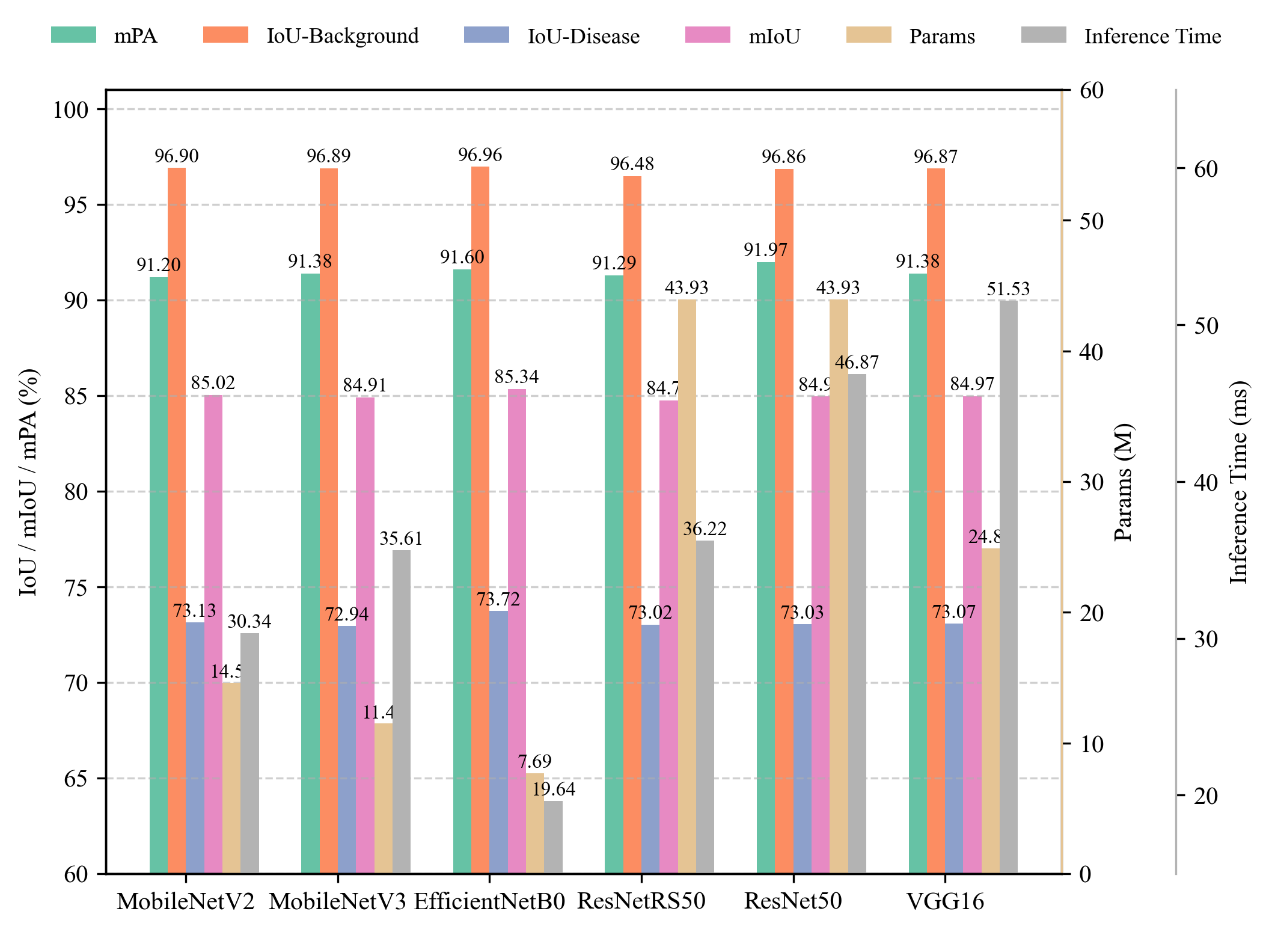
\includegraphics[width=5.76806in,height=4.23611in]{DSLL-Net-media/media/image7.png}

Fig. 7. Performance comparison of U-Net--based lesion segmentation
models using different backbone networks, including VGG16, ResNet50,
ResNetRS50, MobileNetV2, MobileNetV3, and EfficientNet-B0. Models are
evaluated in terms of segmentation accuracy (mPA, IoU-Background,
IoU-Disease, mIoU), parameter count, and inference time.

Fig. 8 compares the performance of the U-Net model with an
EfficientNet-B0 backbone using four attention mechanisms: SE (baseline),
SimAM, ECA, and CBAM. The SE-based model achieved an mPA of 91.60\%,
mIoU of 85.34\%, IoU-Disease of 73.72\%, with 7.69 M parameters and an
inference time of 19.64 ms. Compared with SE, SimAM improved mIoU
(85.46\%) and IoU-Disease (73.94\%) while reducing the parameter count
to 7.05 M, and maintained a competitive inference time (20.55 ms). ECA
achieved the highest mPA (91.94\%) and comparable mIoU (85.22\%), but
required the longest inference time (25.08 ms). CBAM provided marginal
accuracy gains over the baseline but incurred the largest parameter
count (7.99 M) and increased latency (24.07 ms). Overall, SimAM
delivered the most favorable balance between lesion segmentation
accuracy and computational efficiency, and was therefore selected for
subsequent experiments.

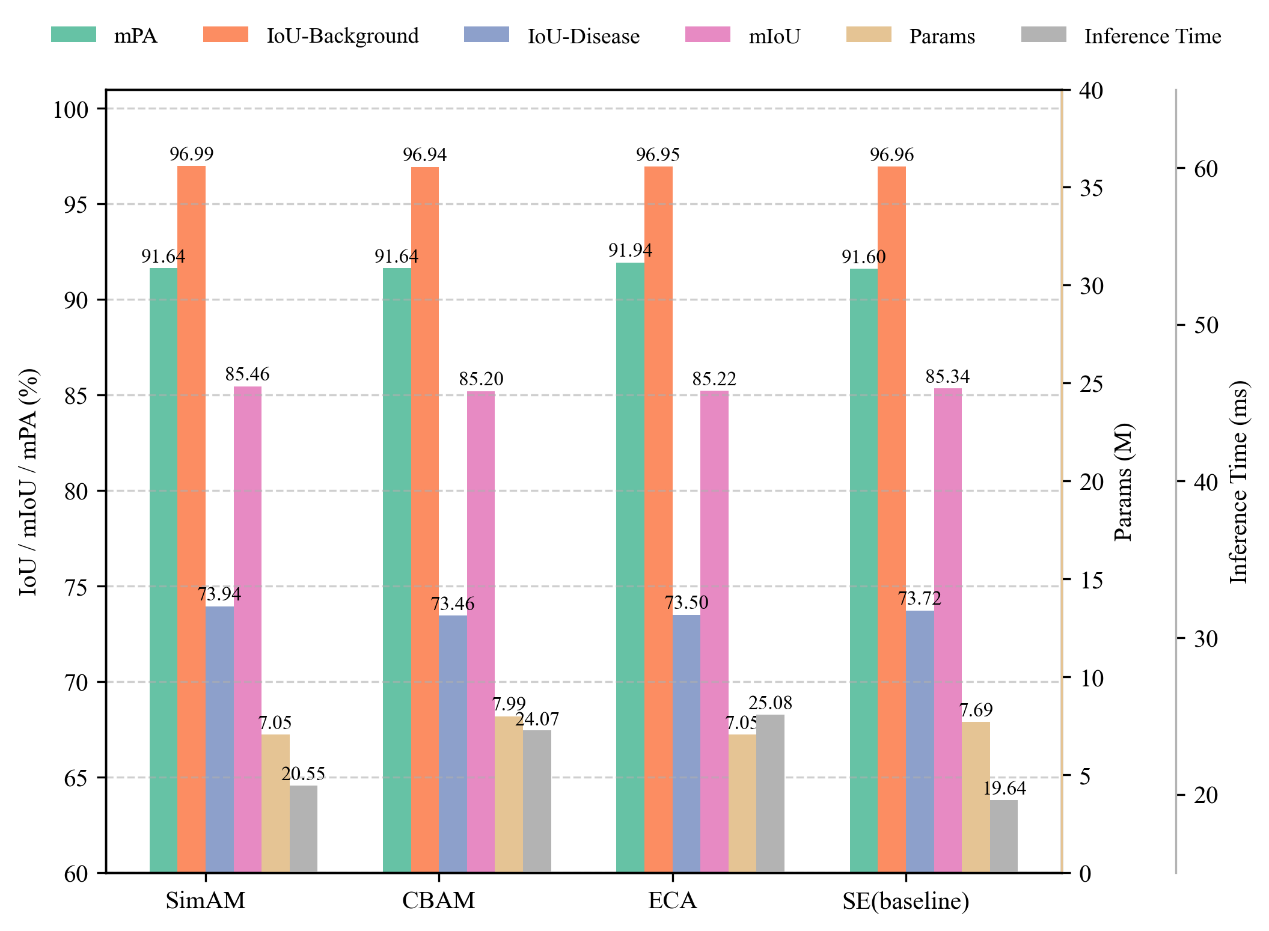
\includegraphics[width=5.76806in,height=4.23611in]{DSLL-Net-media/media/image8.png}

Fig. 8. Performance comparison of U-Net with an EfficientNet-B0 backbone
using different attention mechanisms, including SimAM, CBAM, ECA, and SE
(baseline), evaluated in terms of segmentation accuracy, parameter
count, and inference time.

Fig. 9 compares the lesion segmentation performance of U-Net with an
EfficientNet-B0 backbone using different decoder convolution variants.
RepConv achieved the best overall performance, obtaining the highest
IoU-Disease (74.30\%) and mIoU (85.64\%), with a moderate parameter
count (7.73 M) and the shortest inference time (17.33 ms). CondConv2D
showed competitive accuracy but required more parameters (9.25 M), while
ODConv exhibited the lowest accuracy and the highest computational cost.
The baseline Conv×2 and standard Conv decoders achieved moderate
performance, and PConv, although lightweight, did not provide
competitive accuracy. Overall, RepConv offers the most favorable
trade-off between segmentation accuracy and efficiency and was therefore
adopted in the final model.

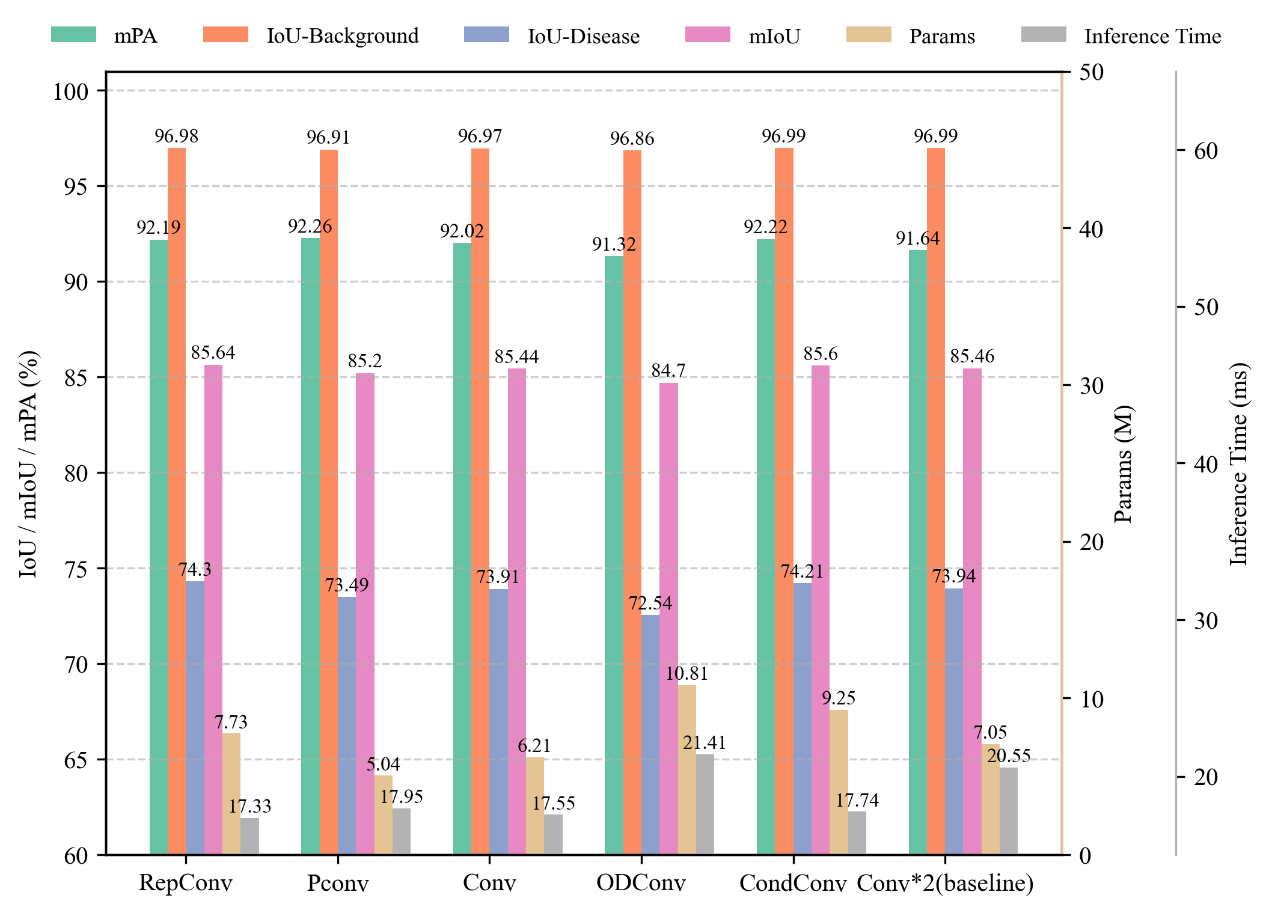
\includegraphics[width=5.76806in,height=4.14653in]{DSLL-Net-media/media/image9.png}

Fig. 9. Lesion segmentation performance of U-Net with a SimAM-enhanced
EfficientNet-B0 backbone using different decoder convolution variants,
including RepConv, PConv, Conv, ODConv, CondConv2D, and Conv×2
(baseline), evaluated in terms of segmentation accuracy, parameter
count, and inference time.

Fig.S1 illustrates the relationship between the SimEffB0-RepUNet
predicted disease severity and the ground truth, in terms of the R²
results and error metrics (MAE and RMSE). The model achieved an
evaluation performance of R² = 0.976, MAE = 0.012, and RMSE = 0.019 on
the test set, demonstrating strong predictive accuracy and robustness in
both disease segmentation and severity quantification tasks.

\hypertarget{model-comparison}{%
\subsection{Model comparison}\label{model-comparison}}

The performance of five single-stage models and two dual-stage models,
including our proposed model, is summarized in Fig. 10. Among the
single-stage models, DeepLabV3+ and U-Net (VGG backbone) ranked the top
two position in both IoU-Leaf (94.44, 92.62) and IoU-Disease (70.9,
70.84) while sharing a much lower inference speed (1138 ms, 1131 ms),
with the former achieving slightly better accuracy and substantially
smaller parameter count than the latter. HRNet performed moderately
across all the metrics. PSPNet achieved a higher accuracy (89.69\% leaf
IoU and 58.88\% disease IoU) only than SegFormer with the smallest
parameter count (2.38 M) and the fastest inference time (392 ms).
SegFormer achieved the lowest leaf IoU (88.59\%) and disease IoU
(55.19\%), with a lightweight architecture (3.71 M) and an inference
time of 361 ms. Compared with the single-stage models, the dual-stage
model achieved substantially higher accuracy while having a relatively
large parameter count and inference time. Among the two dual-stage
models, DeepLabV3+ + U-Net achieved 97.49\% leaf IoU and 72.71\% disease
IoU, with a larger parameter size (32.04 M) and an inference time of
2303 ms. In contrast, the proposed SimV3-DL3+ + SimEffB0-RepUNet model
delivered the best overall performance, attaining 97.76\% leaf IoU and
74.3\% disease IoU while maintaining a moderate parameter size (12.56 M)
and an inference time of 2261 ms.

As observed in Fig.S2, most single-stage models and the DeepLabV3+ +
U-Net pipeline exhibit over-segmentation in leaf extraction, frequently
including background regions and producing boundary inaccuracies along
fine leaf structures. The proposed dual-stage model effectively
mitigates these issues, yielding cleaner leaf masks and more accurate
boundary delineation, which directly contributes to improved lesion
segmentation and disease severity estimation.

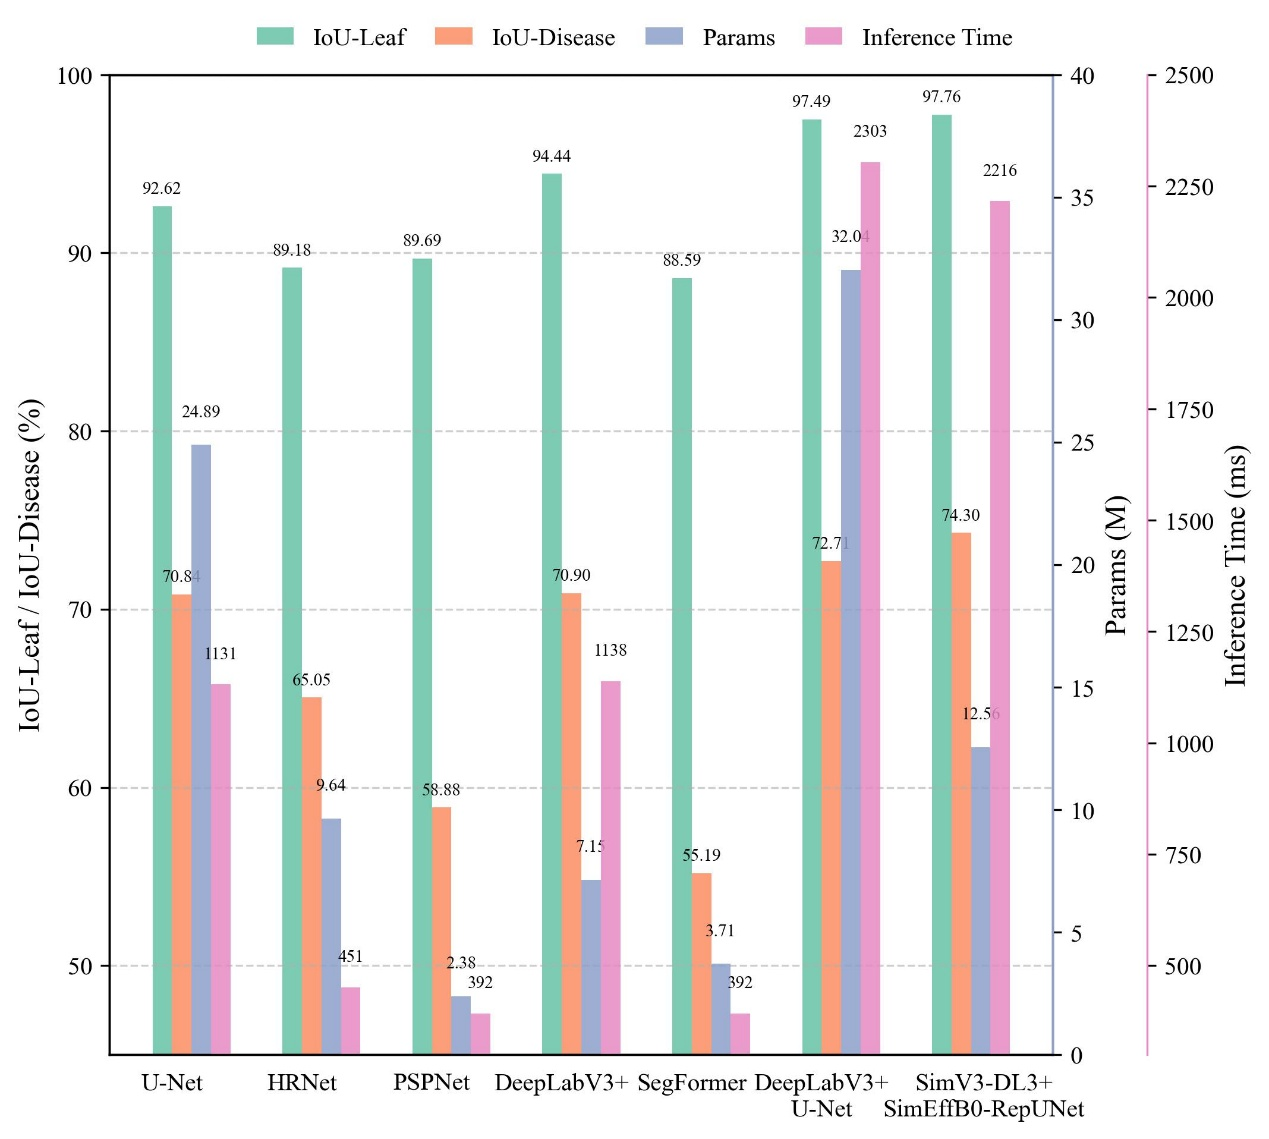
\includegraphics[width=5.76806in,height=5.17708in]{DSLL-Net-media/media/image10.jpeg}

Fig. 10. Performance comparison of segmentation models, including U-Net,
HRNet, PSPNet, DeepLabV3+, SegFormer, DeepLabV3+ + U-Net, and the
proposed SimV3-DL3+ + SimEffB0-RepUNet, evaluated in terms of IoU-Leaf,
IoU-Disease, parameter count, and inference time.

\hypertarget{expert-visual-evaluation-and-model-prediction-1}{%
\subsection{Expert Visual Evaluation and Model
Prediction}\label{expert-visual-evaluation-and-model-prediction-1}}

Fig.S3 compares disease severity estimates provided by 15 trained
technicians. Two representative images with contrasting disease severity
levels were evaluated. For the first image, which exhibited mild disease
symptoms, expert estimates showed noticeable variability and were
consistently higher than the model prediction. The average
expert-estimated severity was 4.56\%, whereas the model predicted a
lower severity of 2.32\%. For the second image, characterized by more
extensive disease symptoms, expert assessments were more concentrated,
with an average estimated severity of 20.01\%, closely aligning with the
model prediction of 19.32\%, despite a few higher individual estimates.

Overall, the comparison indicates that expert visual evaluation tends to
overestimate severity under mild disease conditions, while showing
stronger agreement with model predictions under moderate-to-severe
disease levels. These results highlight the inherent subjectivity and
inter-observer variability in visual severity assessment and demonstrate
the potential of the proposed model to provide more consistent and
objective severity quantification.

\hypertarget{discussion}{%
\section{Discussion}\label{discussion}}

Accurate and quantitative assessment of foliar disease severity is a
core requirement for evaluating yield impacts, screening host
resistance, assessing fungicide efficacy, and supporting evidence-based
disease management across a wide range of crop protection systems.
However, severity estimation from field imagery remains challenging due
to heterogeneous backgrounds, variable illumination, occlusion, and the
coexistence of leaf- and lesion-scale visual patterns. In this study, we
propose a general dual-stage segmentation framework for disease severity
quantification, and demonstrate its effectiveness using grapevine downy
mildew as a representative application scenario. By explicitly
decoupling leaf segmentation and lesion segmentation, the proposed
framework achieves improved boundary delineation, enhanced robustness,
and favorable accuracy--efficiency trade-offs compared with conventional
single-stage approaches.

\textbf{Attention-guided lightweight leaf segmentation for robust field
conditions}

Experimental results demonstrate that the proposed leaf segmentation
model---DeepLabV3+ equipped with a SimAM-enhanced MobileNetV3
backbone---achieves superior segmentation accuracy while simultaneously
reducing model complexity under field conditions (Fig. 4 and Fig. 5).
These improvements can be attributed to the complementary effects of the
lightweight backbone and the parameter-free SimAM attention mechanism
combined with the multiscale context aggregation capability of
DeepLabV3+. Specifically, SimAM enhances spatial sensitivity, enabling
the network to better emphasize salient structural features of leaves
while suppressing background interference, which leads to more accurate
boundary delineation and reduced over-segmentation, as qualitatively
illustrated in Fig.S2. Similar benefits of spatial attention for leaf
segmentation have been reported by Dong et al. {[}35{]}. On the other
hand, owing to the lightweight nature of both MobileNetV3 and SimAM,
incorporating the SimAM attention module into the MobileNetV3 backbone
maintains computational efficiency while enhancing feature
representation. Similarly, Wen et al. {[}36{]} also confirmed the
benefits from the combination of lightweight architecture and attention
mechanism for leaf segmentation. These advantages are critical not only
for improving accuracy in downstream tasks, including lesion detection
and severity estimation, where segmentation accuracy directly impacts
diagnostic reliability, but also for enabling practical deployment in
agricultural settings with limited computational resources.

Overall, the high performance of our model for leaf segmentation
highlights the dual benefits of employing attention-guided lightweight
backbones: improved robustness under diverse illumination and background
conditions, and reduced computational resources consumption that is
essential for practical deployment {[}37-38{]}.

\hypertarget{lesion-segmentation-model-performance-enhancement}{%
\subsection{Lesion segmentation model performance
enhancement}\label{lesion-segmentation-model-performance-enhancement}}

For lesion segmentation, our U‑Net variant employing a SimAM‑enhanced
EfficientNet‑B0 encoder and a RepConv decoder achieved the highest
IoU‑Disease and mIoU (Fig. 6-Fig. 9). Compared with the baseline U-Net,
this model demonstrates a clear improvement in both segmentation
accuracy and computational efficiency. These gains can be primarily
attributed to the combined effects of (i) a lightweight yet expressive
backbone (EfficientNet-B0), (ii) spatial attention via SimAM, and (iii)
structural re-parameterization through RepConv in the decoder.

EfficientNet-B0, designed using compound scaling of depth, width, and
resolution, provides a strong balance between representational capacity
and efficiency {[}39{]}. When integrated into the U-Net encoder,
EfficientNet-B0 enhances multi-scale feature extraction and fusion for
lesion regions without increasing model size. However, its original
squeeze-and-excitation (SE) attention focuses mainly on channel
dependencies and offers limited spatial sensitivity, which can be
suboptimal for segmenting small, irregular, and spatially heterogeneous
disease lesions {[}40{]}. By replacing SE with SimAM, a parameter-free
spatial attention mechanism, the backbone gains enhanced sensitivity to
lesion morphology and spatial distribution, improving lesion
localization while maintaining a lightweight structure
{[}15{]}\textbf{.} This is consistent with the attention comparison
results in Fig. 8, where SimAM provides the most favorable
accuracy--efficiency trade-off among evaluated attention mechanisms.

In the decoder stage, RepConv further strengthens lesion segmentation
performance. During training, RepConv employs a multi-branch structure
that improves feature fusion and boundary refinement, while being
re-parameterized into a single convolutional layer at inference time
{[}27{]} . This design enhances the model's ability to capture
fine-grained lesion boundaries and small lesion regions without
increasing inference complexity. As shown in Fig. 9, the RepConv-based
decoder achieves the highest IoU-Disease and mIoU with the shortest
inference time among all tested convolution variants, highlighting its
suitability for accurate yet efficient lesion segmentation.

Together, the combination of EfficientNet-B0, SimAM, and RepConv allows
the model to focus more effectively on lesion regions while suppressing
irrelevant background signals, leading to substantially higher
segmentation accuracy compared with the baseline U-Net. At the same
time, the use of lightweight attention and structural optimization
reduces the overall parameter count, ensuring that computational
efficiency is maintained without sacrificing predictive power.

Related studies have also demonstrated the effectiveness of enhanced
feature extraction and attention mechanisms in U-Net--based
architectures. For example, Zhang et al. {[}41{]} proposed a U-Net
variant for real-world pest segmentation by incorporating multiscale
feature extraction and attention-based feature fusion, achieving high
segmentation accuracy. However, their work did not explicitly address
lightweight architectural design or efficiency optimization. Similarly,
Gu and Liu {[}42{]} developed a high-performance U-Net for crop disease
segmentation, but computational efficiency and inference time were not
reported. In contrast, the proposed lesion segmentation model explicitly
balances accuracy, efficiency, and deploy ability, making it more
suitable for large-scale and field-oriented applications.

Overall, the lesion segmentation stage of the proposed framework
demonstrates strong adaptability to the complex visual variability of
disease symptoms in real-world vineyard environments, while also
providing a practical foundation for scalable deployment in precision
viticulture and, more broadly, quantitative foliar disease severity
assessment.

\hypertarget{performance-of-the-dual-stage-model}{%
\subsection{Performance of the dual-stage
model}\label{performance-of-the-dual-stage-model}}

Our comparative experiments confirm that dual‑stage models outperform
single‑stage models both in leaf and lesion segmentation accuracy (Fig.
10). This can be attributed to the fact that dual-stage architectures
leverage task decomposition, allowing independent optimization of leaf
and lesion segmentation{[}43{]}. In our dual-stage framework, the
DeepLabV3+ model---optimized for leaf segmentation---exhibited stronger
performance on large and medium-scale targets, effectively delineating
complex leaf boundaries. Meanwhile, the lesion segmentation model
achieved superior accuracy in identifying small lesions and demonstrated
high performance in grape downy mildew segmentation, showing a clear
advantage in capturing subtle and irregular lesion regions. This
architectural decoupling allows each model to specialize in learning
scale- and texture-specific representations, thereby mitigating
interference between structurally distinct targets. These findings
further confirm the effectiveness and suitability of the proposed
dual-stage architecture for complex agricultural scenarios, consistent
with observations reported in recent studies {[}16, 22{]}. In contrast,
single-stage models, while generally more efficient and suitable for
real-time applications, often exhibit divergent performance across leaf
and lesion segmentation tasks. They struggle to achieve optimal results
for both simultaneously, particularly in complex field environments
where occlusion, variable illumination, and background clutter impede
reliable disease detection {[}49-50{]}. Between the two dual-stage
models, our approach strengthens feature extraction and fusion while
maintaining a lightweight architecture, thereby achieving improved
overall performance. This improvement leads to more accurate disease
severity estimation, which is critical for guiding timely and effective
disease management strategies in vineyards. Nevertheless, it should be
noted that the overall performance of dual-stage models is inherently
constrained by the first-stage model, even when the second-stage model
achieves excellent performance. In this regard, the strong performance
of our first-stage model plays a key role in enabling our method to
outperform competing approaches.

\hypertarget{practical-deployment-and-applications}{%
\subsection{Practical deployment and
applications}\label{practical-deployment-and-applications}}

To facilitate field deployment and highlight the real-world
applicability of the proposed dual-stage model, a Flutter-based Android
application was developed
(\url{https://github.com/husnxjsjsb/Grape-Downy} ). The application
integrates the model into a portable, user-friendly platform, enabling
efficient, real-time operation in agricultural environments and
substantially reducing manual labor requirements. This practical
implementation bridges the gap between advanced deep learning algorithms
and on-site agricultural decision-making, aligning with recent progress
in intelligent agriculture {[}21-22{]}. Fig.S4 illustrates the
application's intuitive interface and user interaction. Field deployment
and evaluation verify the model's feasibility under practical
conditions, confirming its robustness, reliability, and scalability. The
demonstration further highlights how lightweight yet accurate models can
provide real-time disease severity assessment, supporting timely
interventions and data-driven crop management. Overall, these findings
demonstrate the model's readiness for broad agricultural deployment and
future system integration.

\hypertarget{limitations}{%
\subsection{Limitations}\label{limitations}}

Despite its advantages, DSLL‑Net still involves two networks and
therefore incurs longer inference times than some single‑stage models.
Model compression or neural architecture search could further reduce
latency. Our evaluation is limited to a single disease and crop; broader
validation across multiple crops, diseases and environments is
necessary. Moreover, pixel‑level annotations remain labor-intensive;
semi‑supervised, weakly supervised or synthetic data approaches could
alleviate this burden. Finally, severity estimation is based solely on
the ratio of lesion to leaf area; integrating temporal progression
models or multispectral data may provide more robust severity
assessments. Addressing these limitations will enhance the scalability
and applicability of quantitative disease severity assessment in
precision agriculture.

\hypertarget{conclusion}{%
\section{Conclusion}\label{conclusion}}

This study proposes a robust and efficient dual-stage architecture for
assessing the severity of grape downy mildew, built upon two
segmentation models: SimV3-DL3+ and SimEffB0-RepUNet. SimV3-DL3+ adopts
a SimAM attention enhanced MobileNetV3 as backbone of DeepLabV3 to
balance segmentation accuracy and computational efficiency for leaf
segmentation, while SimEffB0-RepUNet is a U-Net with a SimAM
enhanced\_EfficientNetB0 as backbone, and a RepConv modules enhanced
decoder. The proposed dual-stage model achieved an IoU-Disease of 74.3\%
in lesion segmentation, demonstrating high accuracy in delineating
diseased regions on grape leaves. With only 12.56 million parameters, it
remains lightweight and well-suited for deployment on mobile or edge
devices. The model also achieved an R² of 0.976 in disease severity
regression, confirming its reliability in quantifying infection levels.
Overall, it provides a compact and high-precision solution for
intelligent assessment of grape downy mildew severity and supports
practical applications in smart agriculture. Future work will expand the
dataset to include grape leaves at various growth stages and under
diverse environmental conditions to further improve the model's
generalization ability. Additionally, we plan to explore approaches for
simultaneous multi-leaf assessment and rapid evaluation to enhance
efficiency in field applications.

\hypertarget{data-and-code-availability}{%
\section{Data and code availability}\label{data-and-code-availability}}

The data and code used in this study are available on GitHub (
\href{https://github.com/husnxjsjsb/Grape-Downy}{https://github.com/}).

\hypertarget{author-contribution-statement}{%
\section{Author contribution
statement}\label{author-contribution-statement}}

Changqing Yan, Gang Zhao: Writing -- review \& editing, Validation,
Supervision, Resources, Project administration, Methodology, Funding
acquisition, Conceptualization. Shuyang Li: Writing -- original draft,
Visualization, Validation, Methodology, Data curation,
Conceptualization. Ling Yin: Supervision, project administration,
funding acquisition. Zhe Liu, Shumei Wei, Xin Lin, Xin Li, Jindong Liu,
Zhenpeng Huang, Danni Zheng, Zeyun Liang, Linjia Yao, Bin Chen, Qi Tian:
Data curation, Investigation, Validation, Writing -- review \& editing.
Chenliang Wang, Junjie Qu: Writing -- review \& editing, Visualization,
Validation, Data curation.

\hypertarget{declaration-of-competing-interest}{%
\section{Declaration of competing
interest}\label{declaration-of-competing-interest}}

The authors declare that they have no known competing financial
interests or personal relationships that could have appeared to
influence the work reported in this paper.

\hypertarget{acknowledgments}{%
\section{Acknowledgments}\label{acknowledgments}}

The authors gratefully acknowledge financial support from the Key
Research and Development Program of Shaanxi (Grant No. 2023-ZDLNY-64),
Guangxi Key R\&D Program Project (Grant No. Gui Ke AB24010121).

\hypertarget{supplementary-materials}{%
\section{Supplementary Materials}\label{supplementary-materials}}

Figs.S1-Figs.S4: Fig.S1 Fig.S2 Fig.S3 Fig.S4.

\hypertarget{references}{%
\section{References}\label{references}}

{[}1{]} L. Guo \emph{et al.}, ``Super pangenome of Vitis empowers
identification of downy mildew resistance genes for grapevine
improvement,'' \emph{Nature Genetics}, vol. 57, no. 3, pp. 741--753,
Mar. 2025, doi: 10.1038/s41588-025-02111-7.{[}2{]} L. Bin, Z. Ding, L.
Tian, D. He, S. Li, and H. Wang, ``Grape Leaf Disease Identification
Using Improved Deep Convolutional Neural Networks,'' \emph{Frontiers in
Plant Science}, vol. 11, p. 1082, Jul. 2020, doi:
10.3389/fpls.2020.01082.{[}3{]} W. Hui \emph{et al.}, ``Adoption of
Sobol's analysis method improved the application of a coupled primary
and secondary infection grape downy mildew model in northern China,''
\emph{Computers and Electronics in Agriculture}, vol. 199, p. 107154,
2022, doi: https://doi.org/10.1016/j.compag.2022.107154.{[}4{]} S.
Savary, A. Ficke, J.-N. Aubertot, and C. Hollier, ``Crop losses due to
diseases and their implications for global food production losses and
food security,'' \emph{Food security}, vol. 4, no. 4, pp. 519--537,
2012.{[}5{]} Y. Wang \emph{et al.}, ``High-efficiency fungicide
screening and field control efficacy of maize southern corn rust,''
\emph{Crop Protection}, vol. 187, p. 106997, 2025.{[}6{]} M. Ji, L.
Zhang, and Q. Wu, ``Automatic grape leaf diseases identification via
UnitedModel based on multiple convolutional neural networks,''
\emph{Information Processing in Agriculture}, vol. 7, no. 3, pp.
418--426, 2020, doi: https://doi.org/10.1016/j.inpa.2019.10.003.{[}7{]}
N. R. Kolhalkar and V. L. Krishnan, ``Mechatronics system for diagnosis
and treatment of major diseases in grape vineyards based on image
processing,'' \emph{Materials Today: Proceedings}, vol. 23, pp.
549--556, 2020, doi: https://doi.org/10.1016/j.matpr.2019.05.407.{[}8{]}
L. I. Cazón, J. A. Paredes, N. R. González, E. C. Conforto, L. Suarez,
and E. M. Del Ponte, ``Optimizing visual estimation of peanut late leaf
spot severity with online training sessions and standard area
diagrams,'' \emph{European Journal of Plant Pathology}, pp. 1--15,
2025.{[}9{]} T. Shi \emph{et al.}, ``Recent advances in plant disease
severity assessment using convolutional neural networks,''
\emph{Scientific Reports}, vol. 13, no. 1, p. 2336, Feb. 2023, doi:
10.1038/s41598-023-29230-7.{[}10{]} K. Li, L. Zhang, B. Li, S. Li, and
J. Ma, ``Attention-optimized DeepLab V3\,+\,for automatic estimation of
cucumber disease severity,'' \emph{Plant Methods}, vol. 18, no. 1, p.
109, Sep. 2022, doi: 10.1186/s13007-022-00941-8.{[}11{]} J. G. M.
Esgario, R. A. Krohling, and J. A. Ventura, ``Deep learning for
classification and severity estimation of coffee leaf biotic stress,''
\emph{Computers and Electronics in Agriculture}, vol. 169, p. 105162,
2020, doi: https://doi.org/10.1016/j.compag.2019.105162.{[}12{]} I.
Hernández \emph{et al.}, ``Assessment of downy mildew in grapevine using
computer vision and fuzzy logic. Development and validation of a new
method,'' \emph{OENO One}, vol. 56, no. 3, pp. 41--53, Jul. 2022, doi:
10.20870/oeno-one.2022.56.3.5359.{[}13{]} Q. Liang, S. Xiang, Y. Hu, G.
Coppola, D. Zhang, and W. Sun, ``PD2SE-Net: Computer-assisted plant
disease diagnosis and severity estimation network,'' \emph{Computers and
Electronics in Agriculture}, vol. 157, pp. 518--529, 2019, doi:
https://doi.org/10.1016/j.compag.2019.01.034.{[}14{]} Z. Wang, L. Yang,
R. Wang, L. Lei, H. Ding, and Q. Yang, ``WE-DeepLabV3+: A lightweight
segmentation model for Panax notoginseng leaf diseases,''
\emph{Computers and Electronics in Agriculture}, vol. 227, p. 109612,
2024, doi: https://doi.org/10.1016/j.compag.2024.109612.{[}15{]} C. Zhao
\emph{et al.}, ``Plant Disease Segmentation Networks for Fast Automatic
Severity Estimation Under Natural Field Scenarios,'' \emph{Agriculture},
vol. 15, no. 6, 2025, doi: 10.3390/agriculture15060583.{[}16{]} I.
Hernández, R. Silva, P. Melo-Pinto, S. Gutiérrez, and J. Tardaguila,
``Early detection of downy mildew in vineyards using deep neural
networks for semantic segmentation,'' \emph{Biosystems Engineering},
vol. 252, pp. 15--31, 2025, doi:
https://doi.org/10.1016/j.biosystemseng.2025.02.007.{[}17{]} L.-C. Chen,
Y. Zhu, G. Papandreou, F. Schroff, and H. Adam, ``Encoder-Decoder with
Atrous Separable Convolution for Semantic Image Segmentation,'' Aug. 22,
2018, \emph{arXiv}: arXiv:1802.02611. doi:
10.48550/arXiv.1802.02611.{[}18{]} V. Iglovikov and A. Shvets,
``TernausNet: U-Net with VGG11 Encoder Pre-Trained on ImageNet for Image
Segmentation,'' 2018, \emph{arXiv}: arXiv:1801.05746. doi:
10.48550/arXiv.1801.05746.{[}19{]} H. Zhao, J. Shi, X. Qi, X. Wang, and
J. Jia, ``Pyramid Scene Parsing Network,'' in \emph{2017 IEEE Conference
on Computer Vision and Pattern Recognition (CVPR)}, 2017, pp.
6230--6239. doi: 10.1109/CVPR.2017.660.{[}20{]} E. Xie, W. Wang, Z. Yu,
A. Anandkumar, J. M. Alvarez, and P. Luo, ``SegFormer: simple and
efficient design for semantic segmentation with transformers,'' in
\emph{Proceedings of the 35th International Conference on Neural
Information Processing Systems}, in NIPS '21. Red Hook, NY, USA: Curran
Associates Inc., 2021.{[}21{]} J. Wang \emph{et al.}, ``Deep
High-Resolution Representation Learning for Visual Recognition,''
\emph{IEEE Transactions on Pattern Analysis and Machine Intelligence},
vol. 43, no. 10, pp. 3349--3364, 2021, doi:
10.1109/TPAMI.2020.2983686.{[}22{]} A. Howard \emph{et al.}, ``Searching
for MobileNetV3,'' in \emph{2019 IEEE/CVF International Conference on
Computer Vision (ICCV)}, 2019, pp. 1314--1324. doi:
10.1109/ICCV.2019.00140.{[}23{]} M. Sandler, A. Howard, M. Zhu, A.
Zhmoginov, and L.-C. Chen, ``MobileNetV2: Inverted Residuals and Linear
Bottlenecks,'' in \emph{2018 IEEE/CVF Conference on Computer Vision and
Pattern Recognition}, 2018, pp. 4510--4520. doi:
10.1109/CVPR.2018.00474.{[}24{]} D. Qin \emph{et al.}, ``MobileNetV4:
Universal Models for Mobile Ecosystem,'' in \emph{Computer Vision --
ECCV 2024: 18th European Conference, Milan, Italy, September 29--October
4, 2024, Proceedings, Part XL}, Berlin, Heidelberg: Springer-Verlag,
2024, pp. 78--96. doi: 10.1007/978-3-031-73661-2\_5.{[}25{]} J. Hu, L.
Shen, and G. Sun, ``Squeeze-and-Excitation Networks,'' in \emph{2018
IEEE/CVF Conference on Computer Vision and Pattern Recognition}, 2018,
pp. 7132--7141. doi: 10.1109/CVPR.2018.00745.{[}26{]} L. Yang, R.-Y.
Zhang, L. Li, and X. Xie, ``SimAM: A Simple, Parameter-Free Attention
Module for Convolutional Neural Networks,'' in \emph{International
Conference on Machine Learning}, 2021. {[}Online{]}. Available:
https://api.semanticscholar.org/CorpusID:235825945{[}27{]} X. Ding, X.
Zhang, N. Ma, J. Han, G. Ding, and J. Sun, ``RepVGG: Making VGG-style
ConvNets Great Again,'' in \emph{2021 IEEE/CVF Conference on Computer
Vision and Pattern Recognition (CVPR)}, 2021, pp. 13728--13737. doi:
10.1109/CVPR46437.2021.01352.{[}28{]} X. Ma, X. Dai, Y. Bai, Y. Wang,
and Y. Fu, ``Rewrite the Stars,'' in \emph{2024 IEEE/CVF Conference on
Computer Vision and Pattern Recognition (CVPR)}, 2024, pp. 5694--5703.
doi: 10.1109/CVPR52733.2024.00544.{[}29{]} K. He, X. Zhang, S. Ren, and
J. Sun, ``Deep Residual Learning for Image Recognition,'' in \emph{2016
IEEE Conference on Computer Vision and Pattern Recognition (CVPR)},
2016, pp. 770--778. doi: 10.1109/CVPR.2016.90.{[}30{]} Q. Wang, B. Wu,
P. Zhu, P. Li, W. Zuo, and Q. Hu, ``ECA-Net: Efficient Channel Attention
for Deep Convolutional Neural Networks,'' in \emph{2020 IEEE/CVF
Conference on Computer Vision and Pattern Recognition (CVPR)}, 2020, pp.
11531--11539. doi: 10.1109/CVPR42600.2020.01155.{[}31{]} S. Woo, J.
Park, J.-Y. Lee, and I. S. Kweon, ``CBAM: Convolutional Block Attention
Module,'' in \emph{Computer Vision -- ECCV 2018: 15th European
Conference, Munich, Germany, September 8--14, 2018, Proceedings, Part
VII}, Berlin, Heidelberg: Springer-Verlag, 2018, pp. 3--19. doi:
10.1007/978-3-030-01234-2\_1.{[}32{]} L. Bai and Z. J. Song,
``Omni-dimensional dynamic convolution with coordinate attention
detection scheme,'' \emph{Science Progress}, vol. 108, no. 2, p.
00368504251336695, 2025, doi: 10.1177/00368504251336695.{[}33{]} J. Chen
\emph{et al.}, ``Run, Don't Walk: Chasing Higher FLOPS for Faster Neural
Networks,'' in \emph{2023 IEEE/CVF Conference on Computer Vision and
Pattern Recognition (CVPR)}, 2023, pp. 12021--12031. doi:
10.1109/CVPR52729.2023.01157.{[}34{]} B. Yang, G. Bender, Q. V. Le, and
J. Ngiam, ``CondConv: conditionally parameterized convolutions for
efficient inference,'' in \emph{Proceedings of the 33rd International
Conference on Neural Information Processing Systems}, Red Hook, NY, USA:
Curran Associates Inc., 2019.{[}35{]} X. Dong \emph{et al.}, ``Detection
of pine wilt disease infected pine trees using YOLOv5 optimized by
attention mechanisms and loss functions,'' \emph{Ecological Indicators},
vol. 168, p. 112764, Nov. 2024, doi:
10.1016/j.ecolind.2024.112764.{[}36{]} F. Wen \emph{et al.}, ``Accurate
recognition and segmentation of northern corn leaf blight in drone RGB
Images: A CycleGAN-augmented YOLOv5-Mobile-Seg lightweight network
approach,'' \emph{Computers and Electronics in Agriculture}, vol. 236,
p. 110433, Sep. 2025, doi: 10.1016/j.compag.2025.110433.{[}37{]} J. Zi,
W. Hu, G. Fan, F. Chen, and Y. Chen, ``SFL-MobileNetV3: A lightweight
network for weed recognition in tropical cassava fields in China,''
\emph{Expert Systems with Applications}, vol. 277, p. 127196, 2025, doi:
https://doi.org/10.1016/j.eswa.2025.127196.{[}38{]} M. Parajuli, M.
Shaban, and T. L. Phung, ``Automated differentiation of skin melanocytes
from keratinocytes in high-resolution histopathology images using a
weakly-supervised deep-learning framework,'' \emph{Int. J. Imaging Syst.
Technol.}, vol. 33, pp. 262-\/-275, 2023, doi:
10.1002/IMA.22810.{[}39{]} C. Lin, P. Yang, Q. Wang, Z. Qiu, W. Lv, and
Z. Wang, ``Efficient and accurate compound scaling for convolutional
neural networks,'' \emph{Neural Networks}, vol. 167, pp. 787--797,
2023.{[}40{]} B. Zhang \emph{et al.}, ``Multi-scale segmentation
squeeze-and-excitation UNet with conditional random field for segmenting
lung tumor from CT images,'' \emph{Computer Methods and Programs in
Biomedicine}, vol. 222, p. 106946, 2022.{[}41{]} C. Zhang, Y. Zhang, and
X. Xu, ``Dilated inception U-Net with attention for crop pest image
segmentation in real-field environment,'' \emph{Smart Agricultural
Technology}, vol. 11, p. 100917, Aug. 2025, doi:
10.1016/j.atech.2025.100917.{[}42{]} R. Gu and L. Liu, ``An agricultural
leaf disease segmentation model applying multi-scale coordinate
attention mechanism,'' \emph{Applied Soft Computing}, vol. 172, p.
112904, Mar. 2025, doi: 10.1016/j.asoc.2025.112904.{[}43{]} C. Wang, P.
Du, H. Wu, J. Li, C. Zhao, and H. Zhu, ``A cucumber leaf disease
severity classification method based on the fusion of DeepLabV3+ and
U-Net,'' \emph{Computers and Electronics in Agriculture}, vol. 189, p.
106373, 2021, doi: https://doi.org/10.1016/j.compag.2021.106373.{[}44{]}
Y. Xu \emph{et al.}, ``Accurate cotton verticillium wilt segmentation in
field background based on the two-stage lightweight DeepLabV3+ model,''
\emph{Computers and Electronics in Agriculture}, vol. 229, p. 109814,
2025, doi: https://doi.org/10.1016/j.compag.2024.109814.{[}45{]} L. G.
Divyanth, A. Ahmad, and D. Saraswat, ``A two-stage deep-learning based
segmentation model for crop disease quantification based on corn field
imagery,'' \emph{Smart Agricultural Technology}, vol. 3, p. 100108,
2023, doi: https://doi.org/10.1016/j.atech.2022.100108.{[}46{]} B.-Y.
Liu, K.-J. Fan, W.-H. Su, and Y. Peng, ``Two-Stage Convolutional Neural
Networks for Diagnosing the Severity of Alternaria Leaf Blotch Disease
of the Apple Tree,'' \emph{Remote Sensing}, vol. 14, no. 11, 2022, doi:
10.3390/rs14112519.{[}47{]} W. Liu \emph{et al.}, ``StripeRust-Pocket: A
Mobile-Based Deep Learning Application for Efficient Disease Severity
Assessment of Wheat Stripe Rust,'' \emph{Plant Phenomics}, vol. 6, p.
0201, 2024, doi: 10.34133/plantphenomics.0201.

\end{document}
